% (c) 2012-2013 Claudio Carboncini - claudio.carboncini@gmail.com
% (c) 2012-2014 Dimitrios Vrettos - d.vrettos@gmail.com
% (c) 2015 Daniele Zambelli daniele.zambelli@gmail.com

\section{Esercizi}

\subsection{Esercizi dei singoli paragrafi}

% \subsubsection*{20.1 - Equazioni di grado superiore al primo riducibili al 
%                 primo grado}
\subsubsection*{\numnameref{sec:compl1_eqgradosup}}

\begin{esercizio}[\Ast]
\label{ese:20.1}
Risolvere le seguenti equazioni riconducendole a equazioni di primo grado.
\begin{multicols}{2}
\begin{enumeratea}
 \item \(x^{2}+2x=0\) \hfill \(\left[0;~-2\right]\)
 \item \(x^{2}+2x-9x-18=0\) \hfill \(\left[-2;~+9\right]\)
 \item \(2x^{2}-2x-4=0\) \hfill \(\left[2;~-1\right]\)
 \item \(4x^{2}+16x+16=0\) \hfill \(\left[-2\right]\)
 \item \(x^{2}-3x-10=0\) \hfill \(\left[5;~-2\right]\)
 \item \(x^{2}+4x-12=0\) \hfill \(\left[2;~-6\right]\)
 \item \(3x^{2}-6x-9=0\) \hfill \(\left[3;~-1\right]\)
 \item \(x^{2}+5x-14=0\) \hfill \(\left[2;~-7\right]\)
 \item \(-3x^{2}-9x+30=0\) \hfill \(\left[2;~-5\right]\)
 \item \(7x^{2}+14x-168=0\) \hfill \(\left[4;~-6\right]\)
%  \item \(x^{4}-16x^{2}=0\) \hfill \(\left[-4;~0;~+4\right]\)
%  \item \(2x^{3}+2x^{2}-20x+16=0\) \hfill \(\left[-4;~+1;~+2\right]\)
%  \item \(-2x^{3}+6x+4=0\) \hfill \(\left[2;~-1\right]\)
%  \item \(-2x^{3}+10x^{2}+82x-90=0\) \hfill \(\left[1;~+9;~-5\right]\)
\end{enumeratea}
\end{multicols}
\end{esercizio}

\begin{esercizio}[\Ast]
\label{ese:20.6}
Risolvere le seguenti equazioni riconducendole a equazioni di primo grado.
\begin{multicols}{2}
\begin{enumeratea}
 \item \(-x^{6}+7x^{5}-10x^{4}=0\) \hfill \(\left[0;~+2;~+5\right]\)
%  \item \(x^{3}-3x^{2}-13x+15=0\) \hfill \(\left[-3;~+1;~+5\right]\)
 \item \(x^{2}+10x-24=0\) \hfill \(\left[-12;~2\right]\)
 \item \(2x^{3}-2x^{2}-24x=0\) \hfill \(\left[-3;~0;~+4\right]\)
 \item \(x^{4}-5x^{2}+4=0\) \hfill \(\left[-2;~-1;~+1;~+2\right]\)
 \item \(-x^{3}-5x^{2}-x-5=0\) \hfill \(\left[-5\right]\)
 \item \(-4x^{4}-28x^{3}+32x^{2}=0\) \hfill \(\left[0;~+1;~-8\right]\)
 \item \(5x^{3}+5x^{2}-80x-80=0\) \hfill \(\left[-1;~+4;~-4\right]\)
 \item \(-3x^{3}+18x^{2}+3x-18=0\) \hfill \(\left[1;~-1;~+6\right]\)
 \item \(4x^{3}+8x^{2}-16x-32=0\) \hfill \(\left[2;~-2\right]\)
%  \item \(x^{3}+11x^{2}+26x+16=0\) \hfill \(\left[-1;~-2;~-8\right]\)
 \item \(2x^{3}+6x^{2}-32x-96=0\) \hfill \(\left[4;~-4;~-3\right]\)
%  \item \(2x^{3}+16x^{2}-2x-16=0\) \hfill \(\left[1;~-1;~-8\right]\)
%  \item \(-2x^{3}+14x^{2}-8x+56=0\) \hfill \(\left[7\right]\)
\end{enumeratea}
\end{multicols}
\end{esercizio}

\begin{esercizio}[\Ast]
\label{ese:20.9}
Risolvere le seguenti equazioni riconducendole a equazioni di primo grado.
\begin{enumeratea}
 \item \(-{\dfrac{3}{2}}x^{2}+\dfrac{3}{2}x+63=0\) \hfill \(\left[7;~-6\right]\)
 \item \(\dfrac{7}{2}x^{2}+7x-168=0\) \hfill \(\left[6;~-8\right]\)
 \item \(\dfrac{3}{4}x^{3}-\dfrac{3}{4}x=0\) \hfill \(\left[0;~+1;~-1\right]\)
 \item \(-{\dfrac{6}{5}}x^{3}-\dfrac{6}{5}x^{2}+\dfrac{54}{5}x+\dfrac{54}{5}=0\) 
  \hfill \(\left[-1;~+3;~-3\right]\)
 \item \(2x^{3}+12x^{2}+18x+108=0\) \hfill \(\left[-6\right]\)
 \item \(x^{4}-10x^{3}+35x^{2}-50x+24=0\) \hfill \(\left[1;~+2;~+3;~+4\right]\)
 \item \(-2x^{3}-12x^{2}+18x+28=0\) \hfill \(\left[-1;~+2;~-7\right]\)
 \item \((x^{2}-6x+8)(x^{5}-3x^{4}+2x^{3})=0\) 
  \hfill \(\left[0;~+1;~+2;~+4\right]\)
 \item \(\left(25-4x^{2}\right)^{4}\left(3x-2\right)^{2}=0\) 
  \hfill \(\left[\frac{5}{2};~-\frac{5}{2};~\frac{2}{3}\right]\)
 \item \((x-4)^{3}\left(2x^{3}-4x^{2}-8x+16\right)^{9}=0\) 
  \hfill \(\left[4;~+2;~-2\right]\)
%  \item \((x^{3}-x)(x^{5}-9x^{3})(x^{2}+25)=0\) 
%   \hfill \(\left[0;~+1;~-1;~+3;~-3\right]\)
%  \item \(x^{5}+3x^{4}-11x^{3}-27x^{2}+10x+24=0\) 
%   \hfill \(\left[1;~-1;~-2;~+3;~-4\right]\)
%  \item \(2x^{2}-x-1=0\) \hfill \(\left[1;~-\frac{1}{2}\right]\)
%  \item \(3x^{2}+5x-2=0\) \hfill \(\left[-2;~\frac{1}{3}\right]\)
%  \item \(-5x^{4}+125x^{2}+10x^{3}-10x-120=0\) \hfill \(\left[1;~-1;~-4;~+6\right]\)
%  \item \(\dfrac{7}{6}x^{4}-\dfrac{161}{6}x^{2}-21x+\dfrac{140}{3}=0\) 
%   \hfill \(\left[1;~-2;~+5;~-4\right]\)
%  \item \(6x^{2}+x-2=0\) \hfill \(\left[\frac{1}{2};~-\frac{2}{3}\right]\)
%  \item \(2x^{3}-x^{2}-2x+1=0\) \hfill \(\left[1;~-1;~\frac{1}{2}\right]\)
%  \item \(3x^{3}-x^{2}-8x-4=0\) \hfill \(\left[-1;~2;~-\frac{2}{3}\right]\)
%  \item \(8x^{3}+6x^{2}-5x-3=0\) 
%   \hfill \(\left[-1;~-\frac{1}{2};~\frac{3}{4}\right]\)
%  \item \(6x^{3}+x^{2}-10x+3=0\) 
%   \hfill \(\left[1;~\frac{1}{3};~-\frac{3}{2}\right]\)
%  \item \(4x^{4}-8x^{3}-13x^{2}+2x+3=0\) 
%   \hfill \(\left[3;~-1;~\frac{1}{2};~-\frac{1}{2}\right]\)
%  \item \(8x^{4}-10x^{3}-29x^{2}+40x-12=0\) 
%   \hfill \(\left[2;~-2;~\frac{3}{4};~\frac{1}{2}\right]\)
%  \item \(-12x^{3}+68x^{2}-41x+5=0\) 
%   \hfill \(\left[5;~\frac{1}{2};~\frac{1}{6}\right]\)
%  \item \((x^{4}+3x^{3}-3x^{2}-11x-6)(4x^{6}-216x^{3}+2916)=0\) 
%   \hfill \(\left[-1;~+2;~+3;~-3\right]\)
\end{enumeratea}
\end{esercizio}

% \subsubsection*{20.2 - Equazioni numeriche frazionarie}
\subsubsection*{\numnameref{sec:compl1_eqfratte}}

\begin{esercizio}[\Ast]
\label{ese:20.15}
Risolvi le seguenti equazioni frazionarie.
\begin{multicols}{2}
\begin{enumeratea}
 \item \(\dfrac{2}{x+1}=\dfrac{1}{x+2}\) \hfill \(\left[-3\right]\)
 \item \(\dfrac{1}{x-1}=2\) \hfill \(\left[\frac{3}{2}\right]\)
 \item \(1-\dfrac{1}{x+1}=0\) \hfill \(\left[0\right]\)
 \item \(\dfrac{2x-4}{x-2}=0\) \hfill \(\left[\emptyset\right]\)
 \item \(\dfrac{x}{x+1}-\dfrac{1}{x-1}=1\) \hfill \(\left[0\right]\)
 \item \(\dfrac{1}{x-3}=\dfrac{x}{3-x}\) \hfill \(\left[-1\right]\)
 \item \(\dfrac{x-1}{x^{2}-4}=-{\dfrac{5}{x+2}}\) 
  \hfill \(\left[\frac{11}{6}\right]\)
 \item \(\dfrac{3}{x+1}=\dfrac{2}{x+1}\) \hfill \(\left[\emptyset\right]\)
 \item \(\dfrac{1}{3-x}-\dfrac{4}{2x-6}=0\) \hfill \(\left[\emptyset\right]\)
 \item \(\dfrac{x^{2}-1}{x-1}-1=2x+1\) \hfill \(\left[-1\right]\)
 \item \(\dfrac{x}{x^{2}-4}=\dfrac{1}{x+2}\) \hfill \(\left[\emptyset\right]\)
 \item \(\dfrac{1}{x}-\dfrac{3}{x^{2}}=\dfrac{2-2x}{x^{3}}\) 
  \hfill \(\left[2;~-1\right]\)
 \item \(\dfrac{x-2}{x-1}=\dfrac{x-1}{x-2}\) \hfill \(\left[\frac{3}{2}\right]\)
 \item \(\dfrac{x+3}{x+1}=x+3\) \hfill \(\left[0;~-3\right]\)
 \item \(\dfrac{3x+1}{3x^{2}+x}=1\) \hfill \(\left[1\right]\)
 \item \(\dfrac{6+x}{x-3}=\dfrac{x^{2}}{x-3}\) \hfill \(\left[-2\right]\)
%  \item \(\dfrac{1}{x-2}+\dfrac{2}{x+1}=\dfrac{3}{x^{2}-x-2}\) 
%   \hfill \(\left[\emptyset\right]\)
%  \item \(\dfrac{5}{x-2}-\dfrac{6}{x+1}=\dfrac{3x-1}{x^{2}-x-2}\)
%   \hfill \(\left[\frac{9}{2}\right]\)
%  \item \(\dfrac{1}{1-x}-\dfrac{x}{x-1}=0\)
%   \hfill \(\left[-1\right]\)
%  \item \(\dfrac{x+1}{x-1}-\dfrac{x}{1+x}=0\)
%   \hfill \(\left[-{\frac{1}{3}}\right]\)
%  \item \(\dfrac{2x+1}{2x-1}+\dfrac{4x^{2}+1}{4x^{2}-1}=2\)
%   \hfill \(\left[-1\right]\)
%  \item \(\dfrac{1}{x-1}+\dfrac{2}{x}+\dfrac{1}{x^{2}-x}=0\)
%   \hfill \(\left[\frac{1}{3}\right]\)
%  \item \(\dfrac{x-1}{x^{2}-2x+1}=\dfrac{2}{2-2x}\)
%   \hfill \(\left[\emptyset\right]\)
%  \item \(4-x^{2}=\dfrac{x^{2}+5x+6}{x+2}-1\)
%   \hfill \(\left[1;~-2\right]\)
\end{enumeratea}
\end{multicols}
\end{esercizio}

\begin{esercizio}[\Ast]
\label{ese:20.21}
Risolvi le seguenti equazioni frazionarie.
\begin{multicols}{2}
\begin{enumeratea}
 \item \(\dfrac{5}{5x+1}+\dfrac{2}{2x-1}=\dfrac{1}{1-2x}\)
  \hfill \(\left[\frac{2}{25}\right]\)
 \item \(\dfrac{1}{x-2}+\dfrac{2}{x+1}=\dfrac{3}{x^{2}-x-2}\)
  \hfill \(\left[\emptyset\right]\)
 \item \(\dfrac{30}{x^{2}-25}+\dfrac{3}{5-x}=0\)
  \hfill \(\left[\emptyset\right]\)
 \item \(\dfrac{x-1}{x+1}=\dfrac{1}{x-2}-\dfrac{1-x^{2}}{x^{2}-x-2}\)
  \hfill \(\left[\frac{1}{2}\right]\)
 \item \(-{\dfrac{3x}{6-2x}}+\dfrac{5x}{10-5x}=\dfrac{1-x}{4-2x}\)
  \hfill \(\left[\frac{3}{4}\right]\)
 \item \(\dfrac{1}{x+3}-\dfrac{1}{2-x}=\dfrac{x+3}{x^{2}+x-6}\)
  \hfill \(\left[\emptyset\right]\)
 \item \(\dfrac{1+2x}{1-2x}+\dfrac{1-2x}{1+2x}=\dfrac{6-8x^{2}}{1-4x^{2}}\)
  \hfill \(\left[\emptyset\right]\)
 \item \(\dfrac{3x}{x-2}+\dfrac{6x}{x^{2}-4x+4}=\dfrac{3x^{2}}{(x-2)^{2}}\)
  \hfill \(\left[\insR-\{2\}\right]\)
 \item \((4x+6)\left(\dfrac{4}{x+1}-\dfrac{1}{x-1}\right)=0\)
  \hfill \(\left[-{\frac{3}{2}};~\frac{5}{3}\right]\)
%  \item \(\dfrac{2x+1}{x+3}+\dfrac{1}{x-4}=\dfrac{4x-9}{x^{2}-x-12}\)
%   \hfill \(\left[1\right]\)
%  \item \(\dfrac{1}{x-1}-\dfrac{1}{x}=\dfrac{(x+1)^{2}}{2(x^{2}-1)}+1\)
%   \hfill \(\left[-{\frac{2}{3}}\right]\)
 \item \(\dfrac{x^{2}-1}{x+1}-\dfrac{1}{x+2}=\dfrac{x+1}{x+2}-x\)
  \hfill \(\left[1\right]\)
%  \item \(\dfrac{1}{x+3}-\dfrac{2}{x+2}=\dfrac{3x-6}{x^{2}+5x+6}\)
%   \hfill \(\left[\frac{1}{2}\right]\)
%  \item \(\dfrac{2x-3}{x+2}+\dfrac{1}{x-4}=\dfrac{2}{x^{2}-2x-8}\)
%   \hfill \(\left[2;~3\right]\)
%  \item \(\dfrac{x-1}{x+2}-\dfrac{x+2}{x-1}=\dfrac{1}{x^{2}+x-2}\)
%   \hfill \(\left[-\frac{2}{3}\right]\)
%  \item \(\dfrac{3}{x-1}+\dfrac{1}{x+1}=\dfrac{12-x}{x^{2}-1}\)
%   \hfill \(\left[2\right]\)
%  \item \(\dfrac{x}{2x+1}+\dfrac{x+1}{2(x+2)}=\dfrac{x-1}{2x^{2}+5x+2}\)
%   \hfill \(\left[\emptyset\right]\)
%  \item \(\dfrac{3x+1}{x^{2}-9}+\dfrac{2}{3x^{2}-9x}=\dfrac{3}{x+3}\)
%   \hfill \(\left[-{\frac{3}{16}}\right]\)
%  \item \(\dfrac{1}{x^{2}-3x+2}+\dfrac{2}{x-1}=0\)
%   \hfill \(\left[\frac{3}{2}\right]\)
%  \item \(\dfrac{x+2}{(x-3)^{2}}-\dfrac{1}{x-3}=\dfrac{4}{9-3x}\)
%   \hfill \(\left[-{\frac{3}{4}}\right]\)
\end{enumeratea}
\end{multicols}
\end{esercizio}

\begin{esercizio}[\Ast]
\label{ese:20.28}
Risolvi le seguenti equazioni frazionarie.
\begin{enumeratea}
 \item \(\dfrac{18x^{2}-9x-45}{4-36x^{2}}-\dfrac{6x+1}{9x-3}+
        \dfrac{21x-1}{18x+6}=0\) \hfill \(\left[\frac{7}{3}\right]\)
 \item \(\dfrac{5x}{3x^{2}-18x+15}-\dfrac{2}{3x-3}=\dfrac{5}{18x-90}\)
  \hfill \(\left[-5\right]\)
 \item \((x-4)(x+3)=\dfrac{(x-4)(x+3)}{x-2}\)
  \hfill \(\left[4;~-3;~3\right]\)
 \item \(\left(\dfrac{1}{x+5}-\dfrac{1}{5}\right):\left(\dfrac{1}{x-5}+
        \dfrac{1}{5}\right)+\dfrac{x^{2}}{x^{2}-5x}=0\)
  \hfill \(\left[\frac{5}{3}\right]\)
 \item \(\dfrac{1}{3x+2}-\dfrac{3}{2-x}=\dfrac{10x+4}{3x^{2}-4x-4}\)
  \hfill \(\left[\insR-\left\{-{\frac{2}{3}};~2\right\}\right]\)
 \item \(\dfrac{1}{2} \left(x-\dfrac{1}{x}\right)-
        2\left(1-\dfrac{1}{x}\right)=\dfrac{x^{2}-1}{x}\)
  \hfill \(\left[-5;~+1\right]\)
 \item \(\dfrac{3(2x-3)}{x^{3}+27}+\dfrac{1}{x+3}=\dfrac{x}{x^{2}-3x+9}\)
  \hfill \(\left[\insR-\{-3\}\right]\)
 \item \(\dfrac{2x-1}{3x^{2}-75}-\dfrac{3-x}{x+5}+\dfrac{x-3}{10-2x}=
        \dfrac{7}{25-x^{2}}\)
  \hfill \(\left[\frac{35}{3}\right]\)
%  \item \(\left(40-10x^{2}\right)^{3} \left(\dfrac{3x-1}{x+2}-
%         \dfrac{3x}{x+1}\right)=0\)
%   \hfill \(\left[2;~-\frac{1}{4};~-2\right]\)
%  \item \(\dfrac{1+2x}{x^{2}+2x}+\dfrac{x^{3}-6x+1}{x^{2}-4}=
%         \dfrac{x^{2}-2x}{x-2}+\dfrac{1}{x^{2}-2x}\)
%   \hfill \(\left[-\frac{4}{3}\right]\)
%  \item \(\left(1-\dfrac{1}{2}x\right):\left(1+\dfrac{1}{2}x\right)=
%         \dfrac{2x+1}{6x+3}-\dfrac{1}{2}x+\dfrac{x^{2}}{2x+4}\)
%   \hfill \(\left[4\right]\)
%  \item \(\dfrac{3x-1}{1-2x}+\dfrac{x}{2x-1}-\dfrac{x^{3}-8}{x^{2}-4}:
%         \dfrac{x^{2}+2x+4}{x^{2}+2x+1}=
%         \dfrac{2-3x}{2x-6}\cdot {\dfrac{x^{2}-9}{4-9x^{2}}}-\dfrac{6x+7}{6}\)
%   \hfill \(\left[-{\frac{26}{25}}\right]\)
%  \item \(\dfrac{2x}{6x-3}+\dfrac{x}{4-8x}+\left(\dfrac{1}{2x+1}-
%         \dfrac{1}{2x-1}\right)\cdot 
%         {\dfrac{2x\left(x^{2}-1\right)}{8x^{2}-4x}}=
%         \dfrac{x^{2}(5x-3)}{3(2x+1)(2x-1)^{2}}\)
%   \hfill \(\left[\frac{12}{5}\right]\)
%  \item \(\dfrac{3x^{2}-2x+3}{x^{2}-3x}+\dfrac{x+2}{3-x}=
%         \left(\dfrac{x+1}{x}-1\right)\left(\dfrac{x^{2}}{x^{3}-27}+
%         \dfrac{x}{x-3}\right):\dfrac{3x}{3x^{3}-81}+\dfrac{x^{2}-x+2}{3-x}\)
%   \hfill \(\left[-30\right]\)
\end{enumeratea}
\end{esercizio}

\begin{esercizio}
\label{ese:20.29}
\(\left(2x-4x^{2}+7\right)^{6}=-{\dfrac{1}{\left(x^{2}-5x+7\right)^{4}}}\) 
Osservando i due membri dell'equazione, senza svolgere i calcoli, puoi subito 
affermare che non esiste alcun numero reale che rende vera l'uguaglianza?
  \hfill \(\left[\right]\)
\end{esercizio}

\begin{esercizio}[\Ast]
\label{ese:20.30}
Quale numero occorre aggiungere a numeratore e denominatore della frazione 
tre settimi perché essa raddoppi di valore?
  \hfill \(\left[21\right]\)
\end{esercizio}

\begin{esercizio}[\Ast]
\label{ese:20.31}
Quale numero occorre aggiungere a numeratore e denominatore della frazione 
due settimi perché essa triplichi di valore?
  \hfill \(\left[28\right]\)
\end{esercizio}

\begin{esercizio}
\label{ese:20.32}
Due amici A e B partono con le loro automobili nello stesso istante da due 
località diverse; A fa un viaggio di \(100\unit{Km}\) a una certa velocità, 
B fa un viaggio di~\(132\unit{Km}\) ad una velocità che supera quella dell'amico 
di~\(20\unit{Km/h}\)
I due amici arrivano nello stesso istante all'appuntamento. 
Qual è la velocità di A?
\begin{center}
 % (c) 2012 Dimitrios Vrettos - d.vrettos@gmail.com
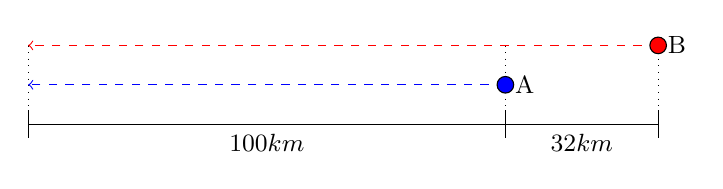
\begin{tikzpicture}[font=\small,x=10mm, y=10mm]
\draw (0,0) -- (8,0);
\foreach \x in {0,6.06,8}{
\draw (\x,5pt) -- (\x,-5pt);
\draw[dotted] (\x,1) -- (\x,0);
}

\draw[dashed, red, ->] (8,1) -- (0,1);
\draw[dashed, blue, ->] (6.06,.5) -- (0,.5);

\draw[fill=blue] (6.06,.5) circle (3pt) node [right] () {A};
\draw[fill=red] (8,1) circle (3pt) node [right] () {B};

\node[below] at (3.03,0) {$100\unit{km}$};
\node[below] at (7.03,0) {$32\unit{km}$};
\end{tikzpicture}
\end{center}
Traccia di soluzione:
\begin{itemize}
 \item se A e B partono insieme e arrivano insieme significa che hanno 
 impiegato lo stesso tempo per fare il proprio viaggio;
 \item il tempo è dato dal rapporto tra lo spazio percorso e la velocità;
 \item la velocità di A è l'incognita del problema: la indichiamo con~\(x\)
 \item l'equazione risolvente è~\(\dfrac{110}{x}=\dfrac{132}{x+20}\)
\end{itemize}
Prosegui nella risoluzione.
\end{esercizio}

\begin{esercizio}
\label{ese:20.33}
Per percorrere~\(480\unit{Km}\) un treno impiega~\(3\) ore di più di quanto 
impiegherebbe un aereo a percorrere~\(1920\unit{Km}\)
L'aereo viaggia ad una velocità media che è~\(8\) volte quella del treno. 
Qual è la velocità del treno?
\end{esercizio}

% \subsubsection*{20.3 - Equazioni letterali}
\subsubsection*{\numnameref{sec:compl1_eqletterali}}

\begin{esercizio}[\Ast]
\label{ese:20.34}
Risolvi e discuti le seguenti equazioni letterali nell'incognita~\(x\)
\begin{enumeratea}
 \item \(1+2x=a+1-2x\)
\hfill \(\left[\forall a\in \insR \rightarrow \left\{\frac{a}{4}\right\}\right]\)
 \item \(2x-\dfrac{7}{2}=ax-5\)
\hfill \(\left[a=2 \rightarrow \emptyset; \quad a \neq~2 \rightarrow 
              \left\{\frac{3}{2(a-2)}\right\}\right]\)
 \item \(b^{2}x=2b+bx\)
\hfill \(\left[b=0 \rightarrow \insR; \quad 
              b=1\rightarrow\emptyset; \quad 
              b\neq~0\wedge b\neq~1\rightarrow \left\{\frac{2}{b-1}\right\}
        \right]\)
 \item \(ax+2=x+3\)
\hfill \(\left[a=1\rightarrow \emptyset; \quad 
              a\neq~1\rightarrow \left\{\frac{1}{a-1}\right\}\right]\)
 \item \(k(x+2)=k+2\)
\hfill \(\left[k=0 \rightarrow \emptyset; \quad k\neq~0 \rightarrow 
\left\{\frac{2-k}{k}\right\}\right]\)
 \item \((b+1)(x+1)=0\)
\hfill \(\left[b=-1 \rightarrow \insR; \quad b\neq -1 \rightarrow 
\left\{-1\right\}\right]\)
 \item \(k^{2}x+2k=x+2\)
\hfill \(\left[k=1 \rightarrow \insR; \quad k=-1 \rightarrow 
\emptyset; \quad k\neq~1\wedge k\neq -1 \rightarrow 
\left\{-{\frac{2}{k+1}}\right\}\right]\)
 \item \((a-1)(x+1)=x+1\)
\hfill \(\left[a=2 \rightarrow \insR; \quad a\neq~2 \rightarrow 
\left\{-1\right\}\right]\)
 \item \(ax+x-2a^{2}-2ax=0\)
  \hfill \(\left[\right]\)
 \item \(3ax-2a=x\cdot (1-2a)+a\cdot (x-1)\)
  \hfill \(\left[\right]\)
%  \item \(x (3-5a)+2 (a-1)=(a-1) (a+1)\)
%   \hfill \(\left[\right]\)
%  \item \(x+2a\cdot (x-2a)+1=0\)
%   \hfill \(\left[\right]\)
%  \item \((a-1)(x+1)=a-1\)
%   \hfill \(\left[a=1 \rightarrow \insR; \quad a\neq~1 \rightarrow \{0\}\right]\)
%  \item \(2k(x+1)-2=k(x+2)\)
%   \hfill \(\left[k=0 \rightarrow \emptyset; \quad 
%   k\neq~0 \rightarrow \left\{\frac{2}{k}\right\}\right]\)
%  \item \(a(a-1)x=2a(x-5)\)
%   \hfill \(\left[a=0 \rightarrow \insR; \quad 
%        a=3\rightarrow \emptyset; \quad 
%        a\neq~0 \wedge a\neq~3 \rightarrow \left\{\frac{10}{3-a}\right\}\right]\)
%  \item \(3ax+a=2a^{2}-3a\)
%   \hfill \(\left[a=0 \rightarrow \insR; \quad 
%           a\neq~0 \rightarrow \left\{\frac{2}{3} (a-2)\right\}\right]\)
% \end{enumeratea}
% \end{esercizio}
% 
% \begin{esercizio}[\Ast]
% \label{ese:20.38}
% Risolvi e discuti le seguenti equazioni letterali nell'incognita~\(x\)
% \begin{enumeratea}
 \item \(3x-a=a(x-3)+6\)
\hfill \(\left[a=3 \rightarrow \insR; \quad a\neq~3 \rightarrow \{2\}\right]\)
 \item \(2+2x=3ax+a-a^{2}x\)
\hfill \(\left[a=2 \rightarrow \insR; \quad 
a=1 \rightarrow \emptyset; \quad 
a\neq~2\wedge a\neq~1 \rightarrow \left\{\frac{1}{a-1}\right\}\right]\)
 \item \(x(a^{2}-4)=a+2\)
\hfill \(\left[a=2 \rightarrow \emptyset; \quad 
a=-2 \rightarrow \insR; \quad 
a\neq -2\wedge a\neq~2 \rightarrow \left\{\frac{1}{a-2}\right\}\right]\)
 \item \((x-m)(x+m)=(x+1)(x-1)\)
\hfill \(\left[m=1\vee m=-1 \rightarrow \insR; \quad 
m\neq~1\wedge m\neq -1 \rightarrow \emptyset\right]\)
 \item \((a-2)^{2}x+(a-2)x+a-2=0\)
\hfill \(\left[a=2 \rightarrow \insR; \quad 
a=1 \rightarrow \emptyset; \quad 
a\neq~1\wedge a\neq~2 \rightarrow \left\{\frac{1}{1-a}\right\}\right]\)
 \item \(\left(9a^{2}-4\right)x=2(x+1)\)
\hfill \(\left[3a^{2}-2=0 \rightarrow \emptyset; \quad 
3a^{2}-2\neq~0 \rightarrow \left\{\frac{2}{3(3a^{2}-2)}\right\}\right]\)
 \item \((a-1)x=a^{2}-1\)
\hfill \(\left[a=1 \rightarrow \insR; \quad 
a\neq~1 \rightarrow \{a+1\}\right]\)
%  \item \((a+2)x=a^{2}+a-1\)
% \hfill \(\left[a=-2 \rightarrow \emptyset; \quad 
% a\neq -2 \rightarrow \left\{\frac{a^{2}+a-1}{a+2}\right\}\right]\)
%  \item \(a(x-1)^{2}=a(x^{2}-1)+2a\)
% \hfill \(\left[a=0 \rightarrow \insR; \quad a\neq~0 \rightarrow \{0\}\right]\)
%  \item \(a^{3}x-a^{2}-4ax+4=0\)
% \hfill \(\left[a=-2\vee a=2 \rightarrow \insR; \quad 
% a=0 \rightarrow \emptyset; \quad 
% a\neq -2\wedge a\neq~0\wedge a\neq~2 \rightarrow 
%   \left\{\frac{1}{a}\right\}\right]\)
%  \item \(bx\left(b^{2}+1\right)-(bx-1)\left(b^{2}-1\right)=2b^{2}\)
% \hfill \(\left[b=0 \rightarrow \emptyset; \quad 
% b\neq~0 \rightarrow \left\{\frac{1+b^{2}}{2b}\right\}\right]\)
%  \item \(a(a-5)x+a(a+1)=-6(x-1)\)
% \hfill \(\left[a=2 \rightarrow \insR; \quad 
% a=3 \rightarrow \emptyset; \quad 
% a\neq~2\wedge a\neq~3 \rightarrow \left\{\frac{a+3}{3-a}\right\}\right]\)
%  \item \((x+a)^{2}-(x-a)^{2}+(a-4)(a+4)=a^{2}\)
% \hfill \(\left[a=0 \rightarrow \emptyset; \quad 
% a\neq~0 \rightarrow \left\{\frac{4}{a}\right\}\right]\)
%  \item \(b(b+3)+x\left(6-b^{2}\right)=bx\)
% \hfill \(\left[b=-3 \rightarrow \insR; \quad 
% b=2 \rightarrow \emptyset; \quad 
% b\neq -3\wedge b\neq~2 \rightarrow \left\{\frac{b}{b-2}\right\}\right]\)
\end{enumeratea}
\end{esercizio}

% \begin{esercizio}[\Ast]
% \label{ese:20.41}
% Risolvi e discuti le seguenti equazioni nell'incognita~\(x\) con due parametri.
% \begin{multicols}{2}
% \begin{enumeratea}
%  \item \((m+1)(n-2)x=0\)
%  \item \(m(x-1)=n\)
%  \item \((a+1)(b+1)x=0\)
%  \item \((m+n)(x-1)=m-n\)
% \end{enumeratea}
% \end{multicols}
% \end{esercizio}
% 
% \begin{esercizio}[\Ast]
% \label{ese:20.42}
% Risolvi e discuti le seguenti equazioni nell'incognita~\(x\) con due parametri.
% \begin{multicols}{2}
% \begin{enumeratea}
%  \item \(x(2a-1)+2b(x-2)=-4a-x\)
%  \item \(ax-3+b=2(x+b)\)
%  \item \((a+1)x=b+1\)
%  \item \((a+b)(x-2)+3a-2b=2b(x-1)\)
% \end{enumeratea}
% \end{multicols}
% \end{esercizio}
% 
% \begin{esercizio}[\Ast]
% \label{ese:20.43}
% Risolvi e discuti le seguenti equazioni nell'incognita~\(x\) con due parametri.
% \begin{enumeratea}
%  \item \(x(x+2)+3ax=b+x^{2}\)
%  \item \((x-a)^{2}+b(2b+1)=(x-2a)^{2}+b-3a^{2}\)
% \end{enumeratea}
% \end{esercizio}
% 
% \begin{esercizio}[\Ast]
% \label{ese:20.44}
% Risolvi e discuti le seguenti equazioni che presentano il parametro al denominatore.
% \begin{multicols}{2}
% \begin{enumeratea}
%  \item \(\dfrac{x+2}{6a}+\dfrac{x-1}{2a^{2}}=\dfrac{1}{3a}\)
%  \item \(\dfrac{x-1}{b}+\dfrac{2x+3}{4b}=\dfrac{x}{4}\)
%  \item \(\dfrac{2x-1}{3a}+\dfrac{x}{3}=\dfrac{2}{a}\)
%  \item \(\dfrac{x}{a}+\dfrac{2x}{2-a}=\dfrac{a-x+2}{2a-a^{2}}\)
% \end{enumeratea}
% \end{multicols}
% \end{esercizio}
% 
% \begin{esercizio}[\Ast]
% \label{ese:20.45}
% Risolvi e discuti le seguenti equazioni che presentano il parametro al denominatore.
% \begin{multicols}{2}
% \begin{enumeratea}
%  \item \(\dfrac{x}{a-1}+8=4a-\dfrac{x}{a-3}\)
%  \item \(\dfrac{x-1}{a-1}+\dfrac{x+a}{a}=\dfrac{a-1}{a}\)
%  \item \(\dfrac{a^{2}-9}{a+2}x=a-3\)
%  \item \(\dfrac{x+2}{a^{2}-2a}+\dfrac{x}{a^{2}+2a}+\dfrac{1}{a}=\dfrac{2}{a^{2}-4}\)
% \end{enumeratea}
% \end{multicols}
% \end{esercizio}
% 
% \begin{esercizio}[\Ast]
% \label{ese:20.46}
% Risolvi e discuti le seguenti equazioni che presentano il parametro al denominatore.
% \begin{enumeratea}
%  \item \(\dfrac{x+1}{a^{2}+2a+1}+\dfrac{2x+1}{a^{2}-a-2}-\dfrac{2x}{(a+1)(a-2)}+\dfrac{1}{a-2}=0\)
%  \item \(\dfrac{x+1}{a-5}+\dfrac{2x-1}{a-2}=\dfrac{2}{a^{2}-7a+10}\)
%  \item \(\dfrac{x+2}{b-2}+\dfrac{2}{b^{2}-4b+4}+\left(\dfrac{1}{b-2}+\dfrac{x}{b-1}\right)\cdot (b-1)=0\)
%  \item \(\dfrac{3+b^{3}x}{7b^{2}-b^{3}}+\dfrac{(2b^{2}+b)x+1}{b(b-7)}=\dfrac{3b^{2}x+1}{b^{2}}-2x\)
%  \item \(\dfrac{x-2}{t^{2}+3t}+\dfrac{x-1}{t+3}=\dfrac{x-2}{t^{2}}+\dfrac{1}{t+3}\)
%  \item \(\dfrac{x}{2a}+\dfrac{x+1}{1-2a}=\dfrac{1}{a}\)
% \end{enumeratea}
% \end{esercizio}
% 
% \begin{esercizio}[\Ast]
% \label{ese:20.47}
% Risolvi e discuti le seguenti equazioni parametriche frazionarie.
% \begin{multicols}{2}
% \begin{enumeratea}
%  \item \(\dfrac{t-1}{x-2}=2t\)
%  \item \(\dfrac{x+m}{x+1}=1\)
%  \item \(\dfrac{3}{x+1}=2a-1\)
%  \item \(\dfrac{2a-x}{x-3}-\dfrac{ax+2}{9-3x}=0\)
% \end{enumeratea}
% \end{multicols}
% \end{esercizio}
% 
% \begin{esercizio}[\Ast]
% \label{ese:20.48}
% Risolvi e discuti le seguenti equazioni parametriche frazionarie.
% \begin{multicols}{2}
% \begin{enumeratea}
%  \item \(\dfrac{k-1}{x}=\dfrac{2}{k+1}\)
%  \item \(\dfrac{k}{x+1}=\dfrac{2k}{x-1}\)
%  \item \(\dfrac{a-1}{x+3}-\dfrac{a}{2-x}=\dfrac{ax+3a}{x^{2}+x-6}\)
%  \item \(\dfrac{a}{x}=\dfrac{1}{a}\)
% \end{enumeratea}
% \end{multicols}
% \end{esercizio}
% 
% \begin{esercizio}[\Ast]
% \label{ese:20.49}
% Risolvi e discuti le seguenti equazioni parametriche frazionarie.
% \begin{enumeratea}
%  \item \(\dfrac{x-a}{x^{2}-1}-\dfrac{x+3a}{2x-x^{2}-1}=\dfrac{x+5}{x+1}-2\dfrac{x}{(x-1)^{2}}-1\)
%  \item \(\dfrac{3}{1+3x}+\dfrac{a}{3x-1}=\dfrac{a-5x}{1-9x^{2}}\)
%  \item \(\dfrac{2a}{x^{2}-x-2}+\dfrac{1}{3x^{2}+2x-1}=\dfrac{6a^{2}-13a-4}{3x^{3}-4x^{2}-5x+2}\)
%  \item \(\dfrac{a+1}{x+1}-\dfrac{2a}{x-2}=\dfrac{3-5a}{x^{2}-x-2}\)
% \end{enumeratea}
% \end{esercizio}
% 
% \begin{esercizio}[\Ast]
% \label{ese:20.50}
% Risolvi e discuti le seguenti equazioni parametriche frazionarie.
% \begin{multicols}{2}
% \begin{enumeratea}
%  \item \(\dfrac{a}{x+a}=1+a\)
%  \item \(\dfrac{x}{x-a}+\dfrac{1}{x+a}=1\)
%  \item \(\dfrac{x+a}{x-a}=\dfrac{x-a}{x+a}\)
%  \item \(\dfrac{2}{1-ax}+\dfrac{1}{2+ax}=0\)
% \end{enumeratea}
% \end{multicols}
% \end{esercizio}
% 
% \begin{esercizio}[\Ast]
% \label{ese:20.51}
% Risolvi e discuti le seguenti equazioni parametriche frazionarie.
% \begin{multicols}{2}
% \begin{enumeratea}
%  \item \(\dfrac{2}{x-2}+\dfrac{a+1}{a-1}=0\)
%  \item \(\dfrac{1}{x+t}-\dfrac{1}{t+1}=\dfrac{tx}{tx+x+t^{2}+t}\)
%  \item \(\dfrac{tx}{x-2}+\dfrac{t^{2}}{t+1}-\dfrac{t}{x-2}=0\)
%  \item \(\dfrac{2x+1}{2x-1}=\dfrac{2a-1}{a+1}\)
% \end{enumeratea}
% \end{multicols}
% \end{esercizio}
% 
% \begin{esercizio}
% \label{ese:20.52}
% Risolvi e discuti le seguenti equazioni parametriche frazionarie.
% \begin{multicols}{2}
% \begin{enumeratea}
%  \item \(\dfrac{a}{x+1}=\dfrac{3}{x-2}\)
%  \item \(\dfrac{x}{x+1}+\dfrac{x}{x-1}=\dfrac{bx}{1-x^{2}}+\dfrac{a+2x^{2}}{x^{2}-1}\)
%  \item \(\dfrac{2x+1}{x}+\dfrac{2x^{2}-3b^{2}}{bx-x^{2}}=\dfrac{1}{x-b}\)
%  \item \(\dfrac{x-1}{x+a}=2+\dfrac{1-x}{x-a}\)
% \end{enumeratea}
% \end{multicols}
% \end{esercizio}
% 
% \paragraph{20.41.}
% a)~\(m=-1\vee n=2 \rightarrow \insR; \quad m\neq -1\wedge n\neq~2 \rightarrow \{0\}\)
% \protect\\
% b)~\(m=0\wedge n\neq~0 \rightarrow \emptyset; \quad m=0\wedge n=0 \rightarrow \insR; \quad m\neq~0 \rightarrow \left\{\frac{m+n}{m}\right\}\)
% \protect\\
% c)~\(a=-1\vee b=-1 \rightarrow \insR; \quad a\neq -1\wedge b\neq -1 \rightarrow \{0\}\)
% \protect\\ d)~\(m=n=0 \rightarrow \insR; \quad m=-n\neq~0 \rightarrow \emptyset; \quad m\neq -n \rightarrow \left\{\frac{2m}{m+n}\right\}\)
% 
% \paragraph{20.42.}
% a)~\(a=b=0 \rightarrow \insR; \quad a=-b\neq~0 \rightarrow \emptyset; \quad a\neq -b \rightarrow \left\{\frac{2(b-a)}{a+b}\right\}\)
% \protect\\ b)~\(a=2\wedge b=-3 \rightarrow \insR; \quad a=2\wedge b\neq -3 \rightarrow \emptyset; \quad a\neq~2 \rightarrow \left\{\frac{b+3}{a-2}\right\}\)
% \protect\\ c)~\(a=-1\wedge b=-1 \rightarrow \insR; \quad a=-1\wedge b\neq -1 \rightarrow \emptyset; \quad a\neq -1 \rightarrow \left\{\frac{b+1}{a+1}\right\}\)
% \protect\\ d)~\(a=b=0 \rightarrow \insR; \quad a=b\neq~0 \rightarrow \emptyset; \quad a\neq b \rightarrow \left\{\frac{2b-a}{a-b}\right\}\)
% 
% \paragraph{20.43.}
% a)~\(a=-{\frac{2}{3}}\wedge b=0 \rightarrow \insR; \quad a=-{\frac{2}{3}}\wedge b\neq~0 \rightarrow \emptyset; \quad a\neq -{\frac{2}{3}} \rightarrow \left\{\frac{b}{2+3a}\right\}\)
% \protect\\ b)~\(a=0\wedge b=0 \rightarrow \insR; \quad a=0\wedge b\neq~0 \rightarrow \emptyset; \quad a\neq~0 \rightarrow \left\{-{\frac{b^{2}}{a}}\right\}\)
% 
% \paragraph{20.44.}
% a)~\(a=0 \rightarrow\) assurdo; \(a=-3 \rightarrow \emptyset; \quad a\neq~0\wedge a\neq -3 \rightarrow \left\{\frac{3}{a+3}\right\}\)
% \protect\\ b)~\(b=0 \rightarrow\) assurdo; \(b=6 \rightarrow \emptyset; \quad b\neq~0\wedge b\neq~6 \rightarrow \left\{\frac{1}{6-b}\right\}\)
% \protect\\ c)~\(a=0 \rightarrow\) assurdo; \(a=-2 \rightarrow \emptyset; \quad a\neq~0\wedge a\neq -2 \rightarrow \left\{\frac{7}{2+a}\right\}\)
% \protect\\ d)~\(a=0\vee a=2 \rightarrow\) assurdo; \(a=-3 \rightarrow \emptyset; \quad a\neq~0\wedge a\neq~2\wedge a\neq -3 \rightarrow \left\{\frac{a+2}{a+3}\right\}\)
% 
% \paragraph{20.45.}
% a)~\(a=1\vee a=3 \rightarrow\) assurdo; \(a\neq~1\wedge a\neq~3 \rightarrow \{2(a-1)(a-3)\}\),
% \protect\\ b)~\(a=0\vee a=1 \rightarrow\) assurdo; \(a=\frac{1}{2} \rightarrow \emptyset; \quad a\neq~0\wedge a\neq \frac{1}{2}\wedge a\neq~1 \rightarrow \left\{\frac{1}{2a-1}\right\}\)
% \protect\\ c)~\(a=-2 \rightarrow\) assurdo; \(a=-3 \rightarrow \emptyset; \quad a=3 \rightarrow \insR; \quad a\neq -3\wedge a\neq -2\wedge a\neq~3 \rightarrow \left\{\frac{a+2}{a+3}\right\}\)
% \protect\\ d)~\(a=0\vee a=-2\vee a=2 \rightarrow\) assurdo; \(a\neq~0\wedge a\neq -2\wedge a\neq~2 \rightarrow \left\{-{\frac{a}{2}}\right\}\)
% 
% \paragraph{20.46.}
% a)~\(a=2\vee a=-1 \rightarrow\) assurdo; \(a\neq~2\wedge a\neq -1 \rightarrow \left\{\frac{a(a+4)}{2-a}\right\}\)
% \protect\\ b)~\(a=5\vee a=2 \rightarrow\) assurdo; \(a=4 \rightarrow \emptyset; \quad a\neq~5\wedge a\neq~2\wedge a\neq~4 \rightarrow \left\{\frac{1}{3(4-a)}\right\}\)
% \protect\\ c)~\(b=2\vee b=1 \rightarrow\) assurdo; \(b\neq~2\wedge b\neq~1 \rightarrow \left\{\frac{b}{2-b}\right\}\)
% \protect\\ d)~\(b=0\vee b=7\rightarrow\) assurdo; \(b\neq~0\wedge b\neq~7 \rightarrow \left\{-{\frac{1}{2b^{2}}}\right\}\)
% \protect\\ e)~\(t=0\vee t=-3 \rightarrow\) assurdo; \(t^{2}=3 \rightarrow \insR; \quad t\neq~0\wedge t\neq -3\wedge t^{2}\neq~3 \rightarrow \{2\}\)
% \protect\\ f)~\(a=0\vee a=\frac{1}{2} \rightarrow\) assurdo; \(a\neq~0\wedge a\neq \frac{1}{2} \rightarrow \{2-6a\}\)
% 
% \paragraph{20.47.}
% a)~\(t=0\vee t=1 \rightarrow \emptyset; \quad t\neq~0\wedge t\neq~1 \rightarrow \left\{\frac{5t-1}{2t}\right\}\)
% \quad b)~\(m=1 \rightarrow \insR-\{-1\}; \quad m\neq~1 \rightarrow \emptyset\)
% \quad c)~\(a=\frac{1}{2} \rightarrow \emptyset; \quad a\neq \frac{1}{2} \rightarrow \left\{-{\frac{2(a-2)}{2a-1}}\right\}\)
% \protect\\ d)~\(a=3\vee a=\frac{7}{9} \rightarrow \emptyset; \quad a\neq~3\wedge a\neq \frac{7}{9} \rightarrow \left\{\frac{2(3a+1)}{3-a}\right\}\)
% 
% \paragraph{20.48.}
% a)~\(k=-1 \rightarrow\) assurdo; \(k=1 \rightarrow \emptyset; \quad k\neq~1\wedge k\neq -1 \rightarrow \left\{-{\frac{\left(k^2-1\right)}{2}}\right\}\)
% \protect\\ b)~\(k=0 \rightarrow \insR-\{1,-1\}; \quad k\neq~0 \rightarrow \{-3\}\), c)~\(a=1 \rightarrow \insR-\{-3,2\}; \quad a\neq~1 \rightarrow \emptyset\)
% \protect\\ d)~\(a=0 \rightarrow\) assurdo; \(a\neq~0 \rightarrow \left\{a^{2}\right\}\)
% 
% \paragraph{20.49.}
% a)~\(a=-5\vee a=-1\vee a=7 \rightarrow \emptyset; \quad a\neq -5\wedge a\neq -1\wedge a\neq~7 \rightarrow \left\{\frac{-2(a-1)}{a+5}\right\}\)
% \quad b)~\(a=-{\frac{4}{3}}\vee a=\frac{5}{9}\vee a=\frac{13}{3} \rightarrow \emptyset; \quad a\neq -{\frac{4}{3}}\wedge a\neq \frac{5}{9}\wedge a\neq \frac{13}{3} \rightarrow \left\{\frac{3-2a}{4+3a}\right\}\)
% \protect\\ c)~\(a=-{\frac{1}{6}} \rightarrow \insR-\left\{-1,2,\frac{1}{3}\right\}; \quad a=\frac{7}{3}\vee a=4\vee a=1 \rightarrow \emptyset; \quad a\neq -{\frac{1}{6}}\wedge a\neq \frac{7}{3}\wedge a\neq~4\wedge a\neq~1 \rightarrow \{a-2\}\)
% \quad d)~\(a=1\vee a=-3\vee a=3 \rightarrow \emptyset; \quad a\neq -3\wedge a\neq~1\wedge a\neq~3 \rightarrow \left\{\frac{5-a}{1-a}\right\}\)
% 
% \paragraph{20.50.}
% a)~\(a=-1\vee a=0 \rightarrow \emptyset; \quad a\neq -1\wedge a\neq~0 \rightarrow \left\{-{\frac{\ a^{2}}{1+a}}\right\}\)
% \protect\\ b)~\(a=-1\vee a=0 \rightarrow \emptyset; \quad a\neq -1\wedge a\neq~0 \rightarrow \left\{-{\frac{a(a-1)}{a+1}}\right\}\)
% \quad c)~\(a=0 \rightarrow \insR-\{0\}; \quad a\neq~0 \rightarrow \{0\}\)
% \quad d)~\(a=0 \rightarrow \emptyset; \quad a\neq~0 \rightarrow \left\{-{\frac{5}{a}}\right\}\)
% 
% \paragraph{20.51.}
% a)~\(a=1 \rightarrow\) assurdo; \(a=-1 \rightarrow \emptyset; \quad a\neq~1\wedge a\neq -1 \rightarrow \left\{\frac{4}{a+1}\right\}\)
% \protect\\ b)~\(t=-1 \rightarrow\) assurdo; \(t\neq -1 \rightarrow \left\{\frac{1}{t+1}\right\}\)
% \protect\\ c)~\(t=-1 \rightarrow\) assurdo; \(t=0 \rightarrow \insR-\{2\}; \quad t=-{\frac{1}{2}} \rightarrow \emptyset; \quad t\neq -\frac{1}{2}\wedge t\neq -1\wedge t\neq~0 \rightarrow \left\{\frac{3t+1}{2t+1}\right\}\)
% \quad d)~\(a=-1 \rightarrow\) assurdo; \(a=2 \rightarrow \emptyset; \quad a\neq -1\wedge a\neq~2 \rightarrow \left\{\frac{3a}{2(a-2)}\right\}\)

% \subsubsection*{20.4 - Equazioni letterali e formule inverse}
\subsubsection*{\numnameref{sec:compl1_formuleinverse}}

\begin{esercizio}
\label{ese:20.53}
Interesse~\(I\) maturato da un capitale~\(C\), al tasso di interesse annuo~\(i\), 
per un numero di anni~\(t\):
\begin{equation*}
  I=C\cdot i\cdot t
\end{equation*}

Ricava le formule per calcolare:~\(C=\ldots\ldots\ldots\ldots\)\,, \(\quad 
i=\ldots\ldots\ldots\ldots\)\,, \(\quad t =\ldots\ldots\ldots\ldots\)\,.

Se il capitale è~\(12.000\) €, il tasso di interesse~\(3,5\%\), il tempo è di~\(6\) 
anni, calcola~\(I\)
\end{esercizio}

\begin{esercizio}
\label{ese:20.54}
Conversione da gradi Celsius \(C\) a gradi Fahrenheit \(F\):
\begin{equation*}
  C=\frac{5(F-32)}{9}
\end{equation*}

Ricava la formula per calcolare\, \(F=\ldots\ldots\ldots\ldots\)\,.

Calcola il valore di~\(C\) quando~\(F\) vale~\(106\) e il valore di~\(F\) 
quando~\(C\) vale~\(12\)
\end{esercizio}

\begin{esercizio}
\label{ese:20.55}
Valore attuale~\(V_a\) di una rendita che vale~\(V_n\) dopo~\(n\) anni, 
anticipata di~\(t\) anni al tasso di interesse~\(i\):
\begin{equation*}
  V_{a}=V_{n}\cdot (1-i\cdot t)
\end{equation*}

Ricava le formule per calcolare:~\(V_n=\ldots\ldots\ldots\ldots\)\,, \(\quad 
i=\ldots\ldots\ldots\ldots\)\,, \(\quad t =\ldots\ldots\ldots\ldots\)\,.

Se il valore attuale è~\(120.000\) €, il tasso di interesse il~\(2\%\), 
calcola il valore della rendita dopo~\(20\) anni.
\end{esercizio}

\begin{esercizio}
\label{ese:20.56}
Sconto semplice~\(S\), per un montante~\(M\), al tasso di interesse~\(i\), per un 
tempo~\(t\) in anni:
\begin{equation*}
  S=\frac{M\cdot i\cdot t}{1+i\cdot t}
\end{equation*}

Ricava le formule per calcolare:~\(M=\ldots\ldots\ldots\ldots\)\,, \(\quad 
i=\ldots\ldots\ldots\ldots\)\,.

Se lo sconto semplice è~\(12.000\) €, il tempo è~\(12\) anni, il tasso di 
interesse il~\(4,5\%\), calcola il montante.
\end{esercizio}

\begin{esercizio}
\label{ese:20.57}
Superficie~\(S\) di un trapezio di base maggiore~\(B\), base minore~\(b\), 
altezza~\(h\):
\begin{equation*}
  S=\frac{1}{2}\cdot (B+b)\cdot h
\end{equation*}

Ricava le formule per calcolare:~\(B=\ldots\ldots\ldots\ldots\)\,, \(\quad 
b=\ldots\ldots\ldots\ldots\)\,, \(\quad h =\ldots\ldots\ldots\ldots\)\,.

Se la base maggiore è~\(12\unit{cm}\), la base minore~\(8\unit{cm}\), la 
superficie~\(12\unit{cm^2}\), calcola l'altezza del trapezio.
\end{esercizio}

\begin{esercizio}
\label{ese:20.58}
Superficie laterale~\(S_l\) di un tronco di piramide con perimetro della base 
maggiore~\(2p\), perimetro della base minore~\(2p'\), apotema~\(a\)
(attenzione~\(2p\) e~\(2p'\) sono da considerare come un'unica incognita):
\begin{equation*}
  S_{l}=\frac{(2p+2p')\cdot a}{2}
\end{equation*}

Ricava le formule per calcolare:~\(2p=\ldots\ldots\ldots\ldots\)\,, 
\(\quad~2p'=\ldots\ldots\ldots\ldots\)\,, \(\quad a =\ldots\ldots\ldots\)\,.

Se la superficie laterale vale~\(144\unit{cm^2}\), il perimetro della base 
minore~\(12\unit{cm}\) e il perimetro della base maggiore~\(14\unit{cm}\), 
calcola l'apotema.
\end{esercizio}

\begin{esercizio}
\label{ese:20.59}
Volume~\(V\) del segmento sferico a una base di raggio~\(r\) e altezza~\(h\)
\begin{equation*}
  V=\pi \cdot h^{2}\cdot \left(r-\frac{h}{3}\right)
\end{equation*}

Ricava la formula per calcolare~\(r=\ldots\ldots\ldots\ldots\)\,.

Se il volume misura~\(200\unit{cm^3}\) e l'altezza~\(10\unit{cm}\), calcola 
la misura del raggio.
\end{esercizio}

\begin{esercizio}
\label{ese:20.60}
Superficie totale~\(S\) del cono di raggio di base~\(r\) e apotema~\(a\):
\begin{equation*}
  S=\pi \cdot r\cdot (r+a)
\end{equation*}

Ricava la formula per calcolare~\(a=\ldots\ldots\ldots\ldots\)\,.

Se la superficie totale è~\(98\unit{cm^2}\) e il raggio~\(6\unit{cm}\), calcola 
la misura dell'apotema.
\end{esercizio}

\begin{esercizio}
\label{ese:20.61}
Velocità~\(v\) nel moto uniformemente accelerato con velocità iniziale~\(v_0\), 
accelerazione costante~\(a\) dopo un tempo~\(t\):
\begin{equation*}
  v=v_{0}+a\cdot t
\end{equation*}

Ricava le formule per calcolare:~\(v_0=\ldots\ldots\ldots\ldots\)\,, \(\quad 
a=\ldots\ldots\ldots\ldots\)\,, \(\quad t =\ldots\ldots\ldots\ldots\)\,.

Se un corpo è passato in~\(10\) secondi dalla velocità~\(10\unit{m/s}\) alla 
velocità~\(24\unit{m/s}\) qual è stata la sua accelerazione?
\end{esercizio}

\begin{esercizio}
\label{ese:20.62}
Spazio percorso~\(s\) nel moto rettilineo uniformemente accelerato in un 
intervallo di tempo~\(t\), per un corpo che ha posizione iniziale
\(s_0\), velocità iniziale~\(v_0\) e accelerazione~\(a\):
\begin{equation*}
  s=s_{0}+v_{0}\cdot t+\dfrac{1}{2}\cdot a\cdot t^{2}
\end{equation*}

Ricava le formule per calcolare:~\(v_0=\ldots\ldots\ldots\ldots\)\,, \(\quad 
a=\ldots\ldots\ldots\ldots\)\,.

Se un corpo ha percorso~\(100\unit{m}\), partendo dalla posizione iniziale~\(0\), 
accelerazione~\(3\unit{m/s^2}\), in~\(10\) secondi, qual'era la sua velocità 
iniziale?
\end{esercizio}

\begin{esercizio}
\label{ese:20.63}
Formula di Bernoulli relativa al moto di un fluido:
\begin{equation*}
  p+\rho \cdot g\cdot h+\dfrac{1}{2}\rho \cdot v^{2}=k
\end{equation*}

Ricava le formule per calcolare:~\(h=\ldots\ldots\ldots\ldots\)\,, \(\quad 
\rho=\ldots\ldots\ldots\ldots\quad\)\,.
\end{esercizio}

\begin{esercizio}
\label{ese:20.64}
Legge di Gay-Lussac per i gas:
\begin{equation*}
  V=V_{0}\cdot (1+\alpha \cdot t)
\end{equation*}

Ricava le formule per calcolare:~\(V_0=\ldots\ldots\ldots\ldots\)\,, \(\quad 
t=\ldots\ldots\ldots\ldots\)\,.
\end{esercizio}

\begin{esercizio}
\label{ese:20.65}
Equazione di stato dei gas perfetti:
\begin{equation*}
  pV=nRT
\end{equation*}

Ricava le formule per calcolare:~\(V=\ldots\ldots\ldots\ldots\)\,, \(\quad 
t=\ldots\ldots\ldots\ldots\)\,.
\end{esercizio}

\begin{esercizio}
\label{ese:20.66}
Rendimento del ciclo di Carnot:
\begin{equation*}
  \eta =1-\dfrac{T_{1}}{T_{2}}
\end{equation*}

Ricava le formule per calcolare:~\(T_1=\ldots\ldots\ldots\ldots\)\,, \(\quad 
T_2=\ldots\ldots\ldots\ldots\)\,.
\end{esercizio}

\begin{esercizio}
\label{ese:20.67}
Legge di Stevino:
\begin{equation*}
  P_{B}=P_{A}+\rho \cdot g\cdot (z_{A}-z_{B})
\end{equation*}

Ricava le formule per calcolare:~\(\rho=\ldots\ldots\ldots\ldots\)\,, \(\quad 
z_A=\ldots\ldots\ldots\ldots\)\,, \(\quad z_B =\ldots\ldots\ldots\ldots\)\,.
\end{esercizio}

% \newpage %-----------------------------------------

\begin{esercizio}
\label{ese:20.68}
Risolvi le seguenti equazioni rispetto alla lettera richiesta.
\begin{multicols}{2}
\TabPositions{2.5cm}
\begin{enumeratea}
 \item \(y=\dfrac{2-a}{x}\)\hfill\(x=\ldots,\,a=\ldots\)
 \item \(y=2-\dfrac{a}{x}\)\hfill\(x=\ldots,\,a=\ldots\)
 \item \(y=\dfrac{2}{x}-a\)\hfill\(x=\ldots,\,a=\ldots\)
 \item \((a+1)(b-1)x=0\)\hfill\(b=\ldots\)
 \item \(y=-{\dfrac{2-a}{x}}\)\hfill\(x=\ldots,\,a=\ldots\)
 \item \(\dfrac{2x+1}{2x-1}=\dfrac{2k-1}{k+1}\)\hfill\(k=\ldots\)
 \item \(\dfrac{2}{x+2}+\dfrac{a-1}{a+1}=0\)\hfill\(a=\ldots\)
 \item \((m-1)x=m-3\)\hfill\(m=\ldots\)
\end{enumeratea}
\end{multicols}
\end{esercizio}

\begin{esercizio}[\Ast]
\label{ese:20.70}
Risolvi le seguenti equazioni rispetto alla lettera richiesta.
\TabPositions{5cm}
\begin{enumeratea}
 \item \(\dfrac{x}{a+b}+\dfrac{x-b}{a-b}=
        \dfrac{b}{a^{2}-b^{2}}\)\tab\(a=\ldots;\quad x=\ldots\)
  \hfill \(\left[a=\frac{b(b+1)}{2x-b}; \quad x=\frac{b(a+b+1)}{2a}\right]\)
 \item \(\dfrac{2x}{a+b}+\dfrac{bx}{a^{2}-b^{2}}-\dfrac{1}{a-b}=0\)\tab\(a=
        \ldots; \quad b=\ldots\)
  \hfill \(\left[a=\frac{b(x+1)}{2x-1}; \quad b=\frac{a(2x-1)}{x+1}\right]\)
\end{enumeratea}
\end{esercizio}
% 
% %%%%%%%%%%%%%%%%%%%%%%%%%%%%%%%%%%%%%%%%%%%%%%%%%%%%%%%%%%
% % \subsubsection*{22.3 - Sistemi fratti}
% \subsubsection*{\numnameref{sec:compl1_sistemifratti}}
% 
% \begin{esercizio}[\Ast]
%  \label{ese:22.44}
% Verifica l'insieme soluzione dei seguenti sistemi.
% \begin{multicols}{2}
% \begin{enumeratea}
% \item \(\longarray\left\{\begin{array}{l}
% \dfrac{4y+x}{5x}=1\\
% \dfrac{x+y}{2x-y}=2\end{array}\right.\)
%  \hfill \(\left[indeterminato\right]\)
% \item \(\longarray\left\{\begin{array}{l}
% y=\dfrac{4x-9}{12}\\
% {\dfrac{y+2}{y-1}+\dfrac{1+2x}{1-x}+1=0}\end{array}\right.\) 
%  \hfill \(\left[(3;~3)\right]\)
% \item \(\longarray\left\{\begin{array}{l}
% 2+3\dfrac{y}{x}=\dfrac{1}{x}\\
% 3\dfrac{x}{y}-1=\dfrac{-2}{y} \end{array}\right.\)
%  \hfill \(\left[(-\frac{5}{11};~\frac{7}{11}\right]\)
% \item \(\longarray\left\{\begin{array}{l}
% \dfrac{y}{2x-1}=-1\\
% 2\dfrac{x}{y-1}=1\end{array}\right.\)
%  \hfill \(\left[impossibile\right]\)
% \item \(\longarray\left\{\begin{array}{l}
% 3\dfrac{x}{y}-\dfrac{7}{y}=1\\
% 2\dfrac{y}{x}+\dfrac{5}{x}=1\end{array}\right.\)
%  \hfill \(\left[\left(\frac{9}{5};-\frac{8}{5}\right)\right]\)
% \item \(\longarray\left\{\begin{array}{l}
% 2\dfrac{x}{3y}-\dfrac{1}{3y}=1\\
% \dfrac{3}{y+2x}=-1\end{array}\right.\)
%  \hfill \(\left[(-1;~-1)\right]\)
% \item \(\longarray\left\{\begin{array}{l}
% \dfrac{x}{9y}=-{\dfrac{1}{2}}+\dfrac{1}{3y}\\
% 9\dfrac{y}{2x}-1-\dfrac{3}{x}=0\end{array}\right.\)
%  \hfill \(\left[impossibile\right]\)
% \item \(\longarray\left\{\begin{array}{l}
% \dfrac{x}{2-\dfrac{y}{2}-2}=1\\
% \dfrac{x-y}{x+\dfrac{3}{2}y-1}=1\end{array}\right.\)
%  \hfill \(\left[\left(-\frac{1}{5};~\frac{2}{5}\right)\right]\)
% \item \(\longarray\left\{\begin{array}{l}
% \dfrac{\dfrac{x}{2}+\dfrac{2y}{3}-\dfrac{1}{6}}{x+y-2}=6\\
% x+y=1\end{array}\right.\)
%  \hfill \(\left[(39;~-38)\right]\)
% \item \(\longarray\left\{\begin{array}{l}
% \dfrac{x-2y}{4}=\dfrac{\dfrac{x-y}{2}+2x}{4}\\
% \dfrac{x}{\dfrac{y}{3}+1}=1\end{array}\right.\)
%  \hfill \(\left[\left(\frac{3}{4};~-\frac{3}{4}\right)\right]\)
% \item \(\longarray\left\{\begin{array}{l}
% \dfrac{x+3y-1}{x-y}=\dfrac{1}{y-x} \\
% x=2y-10 \end{array}\right.\)
%  \hfill \(\left[(-6;~2)\right]\)
% \item \(\longarray\left\{\begin{array}{l}
% \dfrac{2}{x-2}-\dfrac{3}{y+3}=1\\
% \dfrac{5}{y+3}=\dfrac{6}{2-x}-4\end{array}\right.\)
%  \hfill \(\left[(-2;~-5)\right]\)
% \end{enumeratea}
% \end{multicols}
% \end{esercizio}
% 
% \begin{esercizio}[\Ast]
%  \label{ese:22.47}
% Verifica l'insieme soluzione dei seguenti sistemi.
% \begin{enumeratea}
% \item \(\longarray\left\{\begin{array}{l}
% y-\dfrac{x}{3}+\dfrac{3}{4}=0\\
% \dfrac{2x+1}{1-x}+\dfrac{2+y}{y-1}=-1\end{array}\right.\)
%  \hfill \(\left[\left(-\frac{9}{8};~-\frac{9}{8}\right)\right]\)
% \item \(\longarray\left\{\begin{array}{l}
% x+y=2\\
% y\left(\dfrac{x}{y}+3\right)=4\end{array}\right.\)
%  \hfill \(\left[(1;~1)\right]\)
% \item \(\longarray\left\{\begin{array}{l}
% \dfrac{x}{3}-\dfrac{y}{2}=0\\
% \dfrac{y(y-x-1)}{y+1}+x-y+1=\dfrac{1}{2}\end{array}\right.\)
%  \hfill \(\left[impossibile\right]\)
% \item \(\longarray\left\{\begin{array}{l}
% \dfrac{3x-7y+1}{4x^{2}-9y^{2}}=\dfrac{4}{18y^{2}-8x^{2}}\\
% \dfrac{4(1-3x)^{2}}{2}-y=\dfrac{(12x-5)(6x-y)}{4}+3xy+2\end{array}\right.\)
%  \hfill \(\left[\left(-\frac{3}{17};~\frac{6}{17}\right)\right]\)
% \item \(\longarray\left\{\begin{array}{l}
% \dfrac{2x-3y}{x-2y}-\dfrac{3y-1}{x+5y}=
% \dfrac{2(x^{2}+2xy)-(3y-2)^{2}}{x^{2}+3xy-10y^{2}}\\
% x+y=-19\end{array}\right.\)
%  \hfill \(\left[(-18;~-1)\right]\)
% \item \(\longarray\left\{\begin{array}{l}
% \dfrac{x-3}{x-3y+1}+\dfrac{xy-y}{x-3y-1}=
% \dfrac{x^{2}-3xy+x^{2}y-3xy^{2}+3y^{2}}{x^{2}+9y^{2}-6xy-1}\\
% \dfrac{x-3}{5y-1}-\dfrac{y-3}{1+5y}=
% \dfrac{x+5y^{2}-5xy+2}{1-25y^{2}}\end{array}\right.\)
%  \hfill \(\left[\left(\frac{7}{4};~\frac{1}{2}\right)\right]\)
% \item \(\longarray\left\{\begin{array}{l}
% \dfrac{x-2y}{x^{2}-xy-2y^{2}}-\dfrac{1}{y}=2\\
% \dfrac{4}{y}-\dfrac{5}{x+y}=-9\end{array}\right.\)
%  \hfill \(\left[(2;~-1)\right]\)
% \item \(\longarray\left\{\begin{array}{l}
% {2x-y-11=0}\\
% {\dfrac{y+1}{x-1}+\dfrac{3-y}{5x-5}-\dfrac{2}{3}=0}\end{array}\right.\)
%  \hfill \(\left[\right]\)
% \end{enumeratea}
% \end{esercizio}
% 
% \begin{esercizio}
%  \label{ese:22.49}
% Verifica l'insieme soluzione dei seguenti sistemi.
% \begin{multicols}{2}
% \begin{enumeratea}
% \item \(\longarray\left\{\begin{array}{l}
% {\dfrac{x+1}{x}=\dfrac{y+2}{y-2}}\\
% {\dfrac{3x-1}{3x-2}=\dfrac{1+y}{y-2}}\end{array}\right.\)
% \item \(\longarray\left\{\begin{array}{l}
% {\dfrac{2}{5x-y}=\dfrac{-3}{5y-x}}\\
% {\dfrac{1}{4x-3y}=\dfrac{2x+y-1}{3y-4x}}\end{array}\right.\)
% \item \(\longarray\left\{\begin{array}{l}
% {\dfrac{\sqrt{3}}{x-\sqrt{2}}+\dfrac{2\sqrt{2}}{y-\sqrt{3}}=0}\\
% {\dfrac{1}{x-\sqrt{3}}-\dfrac{\sqrt{6}}{2\left(y+2\sqrt{2}\right)}=0}
% \end{array}\right.\)
% \item \(\longarray\left\{\begin{array}{l}
% {\dfrac{x-y+1}{x+y-1}=2}\\
% {\dfrac{x+y+1}{x-y-1}=-2}\end{array}\right.\)
% \item \(\longarray\left\{\begin{array}{l}
% {\dfrac{2}{x-2}=\dfrac{3}{y-3}}\\
% {\dfrac{1}{y+3}=\dfrac{-1}{2-x}}\end{array}\right.\)
% \end{enumeratea}
% \end{multicols}
% \end{esercizio}
% 
% %%%%%%%%%%%%%%
% 
% % \subsubsection*{22.4 - Sistemi letterali}
% \subsubsection*{\numnameref{sec:compl1_sistemiletterali}}
% 
% \begin{esercizio}[\Ast]
%  \label{ese:22.50}
% Risolvere e discutere il seguente sistema. 
% Per quali valori di~\(a\) la coppia soluzione è formata da numeri reali positivi?
% 
% \(\left\{\begin{array}{l}
% {x+ay=2a}\\
% \dfrac{x}{2a}+y=\dfrac{3}{2}
% \end{array}\right.\)
%  \hfill \(\left[a>0\right]\)
% \end{esercizio}
% 
% \begin{esercizio}
%  \label{ese:22.51}
% Perché se il seguente sistema è determinato la coppia soluzione è accettabile?
% 
% \(\left\{\begin{array}{l}
% 3x-2y=0\\
% \dfrac{2x-y}{x+1}=\dfrac{1}{a}
% \end{array}\right.\)
% \end{esercizio}
% 
% 
% \begin{esercizio}
%  \label{ese:22.52}
% Nel seguente sistema è vero che la coppia soluzione è formata da numeri 
% reali positivi se~\(a>2\)?
% \(\left\{\begin{array}{l}
%  \dfrac{a-x}{a^{2}}+a+\dfrac{y-2a}{a+1}=-1\\
%  2y=x
% \end{array}\right.\)
% \end{esercizio}
% 
% 
% \begin{esercizio}
%  \label{ese:22.53}
% Spiegate perché non esiste alcun valore di~\(a\) per cui la
% coppia~\((0;2)\) appartenga a~\(\IS\) del sistema:
% 
% \(\left\{\begin{array}{l}
% 3x-2y=0\\
% \dfrac{2x-y}{x+1}=\dfrac{1}{a}
% \end{array}\right.\)
% \end{esercizio}
% 
% \begin{esercizio}[\Ast]
%  \label{ese:22.54}
% Nel seguente sistema determinate i valori da attribuire al
% parametro~\(a\) affinché la coppia soluzione accettabile sia formata da
% numeri reali positivi.
% 
% \(\left\{\begin{array}{l}
% \dfrac{y}{x}-\dfrac{y-a}{3}=\dfrac{1-y}{3}\\
% a(x+2)+y=1
% \end{array}\right.\)
%  \hfill \(\left[-\frac{1}{2}<a<\frac{1}{2}\right]\)
% \end{esercizio}
% 
% \begin{esercizio}[\Ast]
%  \label{ese:22.55}
% Risolvere i seguenti sistemi.
%  \begin{enumeratea}
% \item \(\left\{\begin{array}{l}
% x+ay=2a\\
% \dfrac{x}{2a}+y=\dfrac{3}{2}\end{array}\right.\) 
%  \hfill \(\left[a\neq~0\rightarrow (a;1)\right]\)
% \item \(\left\{\begin{array}{l}
% \dfrac{x^{3}-8}{x-2}=x^{2}-3x+y-2\\
% \dfrac{x^{2}-4xy+3y^{2}}{3y-x}=k\end{array}\right.\)
% 
%  \hfill \(\left[k~\neq~14 \quad \vee \quad k~\neq~\frac{6}{7} \rightarrow 
%    \left(\frac{k-6}{4}; \frac{5k-6}{4}\right); \quad 
%  k=14 \quad \vee \quad k=\frac{6}{7} \rightarrow \text{impossibile}\right]\)
% \item \(\left\{\begin{array}{l}
% kx-y=2\\
% x+6ky=0\end{array}\right.\)
%  \hfill \(\left[\forall k \rightarrow 
%   \left(\frac{12k}{6k^{2}+1};~\frac{2}{6k^{2}+1}\right)\right]\)
% \item \(\left\{\begin{array}{l}
% kx-8y=4\\
% 2x-4ky=3\end{array}\right.\)
%  \hfill \(\left[k\neq -2 \vee k\neq~2 \rightarrow 
% \left(\frac{4k-6}{k^{2}-4}; \frac{8-3k}{4(k^{2}-4)}\right);~  
% k=-2 \vee k=2 \rightarrow \text{impossibile}\right]\)
%  \end{enumeratea}
% \end{esercizio}
% 
% \begin{esercizio}[\Ast]
%  \label{ese:22.56}
% Risolvere i seguenti sistemi.
%  \begin{enumeratea}
% \item \(\left\{\begin{array}{l}
% 4x-k^{2}y=k\\
% kx-4ky=-3k\end{array}\right.\)
% 
% \hfill \(\left[ \begin{array}{r} 
% k\neq -4 \vee k\neq~4 \vee k\neq~0 \rightarrow 
%    \left(\frac{3k^{2}+4k}{16-k^{2}};~\frac{k+12}{16-k^{2}}\right) \\
% k=-4 \vee k=4 \rightarrow \text{impossibile} \\
% k=0 \rightarrow \text{ indeterminato con soluzioni tipo}~ 
%    (0;t) \wedge t \in \insR 
% \end{array} \right]\)
%    
% \item \(\left\{\begin{array}{l}
% kx-4ky=-6\\
% kx-k^{2}y=0\end{array}\right.\)
%  \hfill \(\left[k\neq~0 \vee k\neq~4 \rightarrow 
% \left(\frac{6}{4-k}; \frac{6}{k(4-k)}\right); \quad
% k=0\vee k=4 \rightarrow \text{ impossibile}\right]\)
% \item \(\left\{\begin{array}{l}
% (k-1)x+(1-k)y=0\\
% (2-2k)x+y=-1\end{array}\right.\)
% 
% \hfill \(\left[ \begin{array}{r} 
% k\neq~1 \vee k\neq \frac{3}{2} \rightarrow 
%    \left(\frac{1}{2k-3};~\frac{1}{2k-3}\right) \\
% k=\frac{3}{2} \rightarrow \text{ impossibile}; \quad \\
% k=1 \rightarrow \text{ indeterminato con soluzioni tipo }
% (t;-1) \wedge t \in \insR
% \end{array} \right]\)
%  \end{enumeratea}
% \end{esercizio}

% % \subsubsection*{22.5 - Sistemi lineari di tre equazioni in tre incognite}
% \subsubsection*{\numnameref{sec:compl1_sistemitreeq}}
% 
% \begin{esercizio}[\Ast]
%  \label{ese:22.57}
%  Determinare la terna di soluzione dei seguenti sistemi.
% \begin{multicols}{2}
% \begin{enumeratea}
% \item \(\left\{\begin{array}{l}
% x-2y+z=1 \\
% x-y=2 \\
% x+3y-2z=0 \end{array}\right.\)
% \hfill \(\left[(0;~-2;~3)\right]\)
% \item \(\left\{\begin{array}{l}
% x+y+z=4 \\
% x-3y+6z=1\\
% x-y-z=2 \end{array}\right.\)
% \hfill \(\left[\left(3;~\frac{8}{9};~\frac{1}{9}\right)\right]\)
% \item \(\left\{\begin{array}{l}
% x+2y-3z=6-3y\\
% 2x-y+4z=x\\
% 3x-z=y+2\end{array}\right.\)
% \hfill \(\left[(1;~1;~0)\right]\)
% \item \(\left\{\begin{array}{l}
% 2x-y+3z=1 \\
% x-2y+z=5\\
% x+2z=3 \end{array}\right.\)
% \hfill \(\left[(-21;~-7;~12)\right]\)
% \item \(\left\{\begin{array}{l}
% x+2y-z=1 \\
% y-4z=0\\
% x-2y+z=2 \end{array}\right.\)
% \hfill \(\left[\left(\frac{3}{2};~-\frac{2}{7};~-\frac{1}{14}\right)\right]\)
% \item \(\left\{\begin{array}{l}
% x-3y+6z=1 \\
% x+y+z=5 \\
% x+2z=3 \end{array}\right.\)
% \hfill \(\left[(-5;~6;~4)\right]\)
% \item \(\left\{\begin{array}{l}
% x-4y+6z=2 \\x+4y-z=2\\x+3y-2z=2 
% \end{array}\right.\)
% \hfill \(\left[(2;~0;~0)\right]\)
% \item \(\left\{\begin{array}{l}
% 4x-y-2z=1 \\3x+2y-z=4\\x+y+2z=4 
% \end{array}\right.\)
% \hfill \(\left[(1;~1;~1)\right]\)
% \item \(\left\{\begin{array}{l}
% x-3y=3 \\x+y+z=-1\\2x-z=0 
% \end{array}\right.\)
% \hfill \(\left[(0;~-1;~0)\right]\)
% \item \(\left\{\begin{array}{l}
% 2x-y+3z=1 \\x-6y+8z=2\\3x-4y+8z=2 
% \end{array}\right.\)
% \hfill \(\left[\left(\frac{2}{3};~-\frac{2}{3};~-\frac{1}{3}\right)\right]\)
% \item \(\left\{\begin{array}{l}
% 4x-6y-7z=-1 \\x+y-z=1\\3x+2y+6z=1 
% \end{array}\right.\)
% \hfill \(\left[\left(\frac{9}{31};~\frac{17}{31};~-\frac{5}{31}\right)\right]\)
% \item \(\left\{\begin{array}{l}
% 4x-3y+z=4\\x+4y-3z=2 \\y-7z=0 
% \end{array}\right.\)
% \hfill \(\left[\left(\frac{7}{6};~\frac{7}{30};~\frac{1}{30}\right)\right]\)
% \item \(\left\{\begin{array}{l}
% 3x-6y+2z=1 \\x-4y+6z=5\\x-y+4z=10 
% \end{array}\right.\)
% \hfill \(\left[(5;~3;~2)\right]\)
% \item \(\left\{\begin{array}{l}
% 4x-y-7z=-12 \\x+3y+z=-4\\2x-y+6z=5 
% \end{array}\right.\)
% \hfill \(\left[\left(-{\frac{60}{43}};~-\frac{53}{43};~\frac{47}{43}\right)
%         \right]\)
% \item \(\left\{\begin{array}{l}
% 2x+y-5z=2 \\x+y-7z=-2\\x+y+2z=1 
% \end{array}\right.\)
% \hfill \(\left[\left(\frac{10}{3};~-3;~\frac{1}{3}\right)\right]\)
% \item \(\left\{\begin{array}{l}
% 3x-y+z=-1\\x-y-z=3 \\x+y+2z=1 
% \end{array}\right.\)
% \hfill \(\left[(6;~11;~-8)\right]\)
% \item \(\left\{\begin{array}{l}
% x-4y+2z=7 \\-3x-2y+3z=0 \\x-2y+z=1 
% \end{array}\right.\)
% \hfill \(\left[\left(-5;~-\frac{33}{4};~-\frac{21}{2}\right)\right]\)
% \item \(\left\{\begin{array}{l}
% -2x-2y+3z=4 \\2x-y+3z=0\\2x+y=1 
% \end{array}\right.\)
% \hfill \(\left[\left(-{\frac{5}{2}};~6;~\frac{11}{3}\right)\right]\)
% \end{enumeratea}
% \end{multicols}
% \end{esercizio}
% 
% \begin{esercizio}
%  \label{ese:22.60}
% Quale condizione deve soddisfare il parametro~\(a\) affinché il sistema seguente 
% non sia privo di
% significato? Determina la terna soluzione assegnando ad~\(a\) il valore~2.
%  \[\left\{\begin{array}{l}x+y+z=\frac{a^{2}+1}{a}\\ay-z=a^{2} \\
%  y+ax=a+1+a^{2}z\end{array}\right.\]
% \end{esercizio}
% 
% \begin{esercizio}
%  \label{ese:22.61}
% Determina il dominio del sistema e stabilisci se la terna soluzione è 
% accettabile:
% \[\longarray\left\{\begin{array}{l}\frac{5}{1-x}+\frac{3}{y+2}=
% \frac{2x}{xy-2+2x-y}\\
% \frac{x+1-3(y-1)}{\text{xyz}}=\frac{1}{xy}-\frac{2}{yz}-\frac{3}{xz}\\
% x+2y+z=0\end{array}\right.\]
% \end{esercizio}
% 
% \begin{esercizio}
%  \label{ese:22.62}
% Verifica se il sistema è indeterminato:
% \[\left\{\begin{array}{l}x+y=1 \\y-z=5
% \\x+z+2=0 \end{array}\right.\]
% \end{esercizio}
% 
% \begin{esercizio}
%  \label{ese:22.63}
% Determina il volume del parallelepipedo retto avente
% per base un rettangolo, sapendo che le dimensioni della base e
% l'altezza hanno come misura (rispetto al~\(\unit{cm}\)) i valori
% di~\(x, y, z\) ottenuti risolvendo il sistema:
% \[\left\{\begin{array}{l}3x+1=2y+3z \\6x+y+2z=7
% \\9(x-1)+3y+4z=0 \end{array}\right.\]
% \end{esercizio}
% 
% %%%%%%%%%%%%%%%%%%%%%%%%%%%%%%%%%%%%%%%%%%%%

% \subsubsection*{22.6 - Sistemi da risolvere con sostituzioni delle variabili}
\subsubsection*{\numnameref{sec:compl1_sistemisotituzionevariabili}}

\begin{esercizio}[\Ast]
 \label{ese:22.64}
 Risolvi i seguenti sistemi per mezzo di opportune sostituzioni delle variabili.

\begin{enumeratea}
\item \(\longarray\left\{\begin{array}{l}
\dfrac{1}{2x}+\dfrac{1}{y}=-4\\\dfrac{2}{3x}+\dfrac{2}{y}=1
\end{array}\right. 
\qquad \text{sostituire} \quad u=\frac{1}{x} \quad v=\frac{1}{y}\)
\hfill \(\left[\left(-{\frac{1}{27}};~\frac{2}{19}\right)\right]\)

% \item \(\left\{\begin{array}{l}
% x^{2}+y^{2}=13\\x^{2}-y^{2}=5 
% \end{array}\right. 
% \qquad \text{sostituire} u=x^{2} \quad v=y^{2}\)
% \hfill \(\left[(3;2);~(-3;2);~(3;-2);~(-3;-2)\right]\)

\item \(\longarray\left\{\begin{array}{l}
\dfrac{1}{x+y}+\dfrac{2}{x-y}=1\\\dfrac{3}{x+y}-\dfrac{5}{x-y}=2
\end{array}\right. 
\quad \text{sostituire} \quad u=\frac{1}{x+y} \quad v=\ldots\)
\hfill \(\left[\left(\frac{55}{9};~-\frac{44}{9}\right)\right]\)

\end{enumeratea}
\end{esercizio}

\begin{esercizio}[\Ast]
 \label{ese:22.65}
 Risolvi i seguenti sistemi per mezzo di opportune sostituzioni delle variabili.
\begin{multicols}{2}
\begin{enumeratea}
{\longarray
\item \(\left\{\begin{array}{l}
\dfrac{5}{2x}-\dfrac{2}{y}=2\\\dfrac{1}{x}+\dfrac{2}{y}=1
\end{array}\right.\)
\hfill \(\left[\left(\frac{7}{6};~14\right)\right]\)
\item \(\left\{\begin{array}{l}
\dfrac{1}{x}+\dfrac{2}{y}=3\\\dfrac{1}{x}+\dfrac{3}{y}=4
\end{array}\right.\)
\hfill \(\left[\left(1;~1\right)\right]\)
\item \(\left\{\begin{array}{l}
\dfrac{2}{x}+\dfrac{4}{y}=-3\\\dfrac{2}{x}-\dfrac{3}{y}=4 
\end{array}\right.\)
\hfill \(\left[\left(2;~-1\right)\right]\)
\item \(\left\{\begin{array}{l}
\dfrac{1}{x+1}-\dfrac{2}{y-1}=2\\\dfrac{2}{x+1}-\dfrac{1}{y-1}=3
\end{array}\right.\)
\hfill \(\left[\left(-{\frac{1}{4}};~-2\right)\right]\)}
% \end{enumeratea}
% \end{multicols}
% \end{esercizio}
% 
% \begin{esercizio}[\Ast]
%  \label{ese:22.66}
%  Risolvi i seguenti sistemi per mezzo di opportune sostituzioni delle variabili.
% \begin{multicols}{2}
% \begin{enumeratea}
\item \(\longarray\left\{\begin{array}{l}
\dfrac{1}{x}-\dfrac{3}{y}+\dfrac{2}{z}=3 \\
\dfrac{2}{x}-\dfrac{3}{y}+\dfrac{2}{z}=4 \\
\dfrac{2}{x}+\dfrac{4}{y}-\dfrac{1}{z}=-3
\end{array}\right.\)
\hfill \(\left[\left(1;~-\frac{5}{8};~-\frac{5}{7}\right)\right]\)
\item \(\left\{\begin{array}{l}
x^{3}+y^{3}=9 \\2x^{3}-y^{3}=-6 
\end{array}\right.\)
\hfill \(\left[(1;~2)\right]\)
% \item \(\left\{\begin{array}{l}
% x^{2}+y^{2}=-1\\x^{2}-3y^{2}=12
% \end{array}\right.\)
% \hfill \(\left[\emptyset\right]\)
\end{enumeratea}
\end{multicols}
\end{esercizio}

% \begin{esercizio}[\Ast]
%  \label{ese:22.66}
% \(\longarray\left\{\begin{array}{l}
% \dfrac{4}{x^{2}}-\dfrac{2}{y^{2}}-\dfrac{2}{z^{2}}=0\\
% \dfrac{1}{x^{2}}+\dfrac{1}{z^{2}}=2 \\
% \dfrac{2}{y^{2}}-\dfrac{2}{z^{2}}=0
% \end{array}\right.\)
% \hfill \(\left[\begin{array}{r}
% (+1;~+1;~+1); \quad (-1;~+1;~+1) \\
% (+1;~-1;~+1); \quad (+1;~+1;~-1) \\
% (-1;~-1;~+1); \quad (-1;~+1;~-1) \\
% (+1;~-1;~-1); \quad (-1;~-1;~-1)
% \end{array}\right]\)
% \end{esercizio}
% 
% % \subsubsection*{21.4 - Disequazioni polinomiali di grado superiore al primo}
% \subsubsection*{\numnameref{sec:compl1_disequazionipolinomialiefratte}}
% 
% \begin{esercizio}
%  \label{ese:21.42}
% Risolvi le seguenti disequazioni.
% \begin{multicols}{2}
% \begin{enumeratea}
% \item \((x+3)\cdot \left(\frac{1}{5}x+\frac{3}{2}\right) < 0\)
% \item \(\left(-{\frac{6}{11}}+2x\right)\cdot\left(-x+\frac{9}{2}\right) \le 0\)
% \item \((x-3)\cdot (2x-9)\cdot (4-5x) > 0\)
% \item \(\left(x+\frac{3}{2}\right)\cdot \left(5x+\frac{1}{5}\right) < 0\)
% \item \(\left(-{\frac{1}{10}}x+2\right)\cdot \left(-3x+9\right) \ge 0\)
% \item \((4x+3)\cdot (-2x-9)\cdot (-4x+5) > 0\)
% \end{enumeratea}
% \end{multicols}
% \end{esercizio}
% 
% \begin{esercizio}[\Ast]
%  \label{ese:21.44}
% Trovare l'Insieme Soluzione delle seguenti disequazioni.
% \begin{multicols}{2}
%  \begin{enumeratea}
% \item \((x+2)(3-x)\le~0\) \hfill \(\left[x\le -2\vee x\ge~3\right]\)
% \item \(x(x-2)>0\) \hfill \(\left[x<0\vee x>2\right]\)
% \item \((3x+2)(2-3x)<0\) \hfill \(\left[x<-{\frac{2}{3}}\vee x>\frac{2}{3}\right]\)
% \item \((-2x+5)(-3x+7)<0\) \hfill \(\left[\right]\)
% \end{enumeratea}
% \end{multicols}
% \end{esercizio}
% 
% \begin{esercizio}[\Ast]
%  \label{ese:21.45}
% Trovare l'Insieme Soluzione delle seguenti disequazioni.
%  \begin{enumeratea}
% \item \(-3x(2-x)(3-x)\ge~0\) \hfill \(\left[x\ge~0\vee~2\le x\le~3\right]\)
% \item \((x+1)(1-x)\left(\frac{1}{2}x-2\right)\ge~0\) 
%  \hfill \(\left[x\le -1\vee~1\le x\le4\right]\)
% \item \((x-1)(x-2)(x-3)(x-4)<0\) \hfill \(\left[1<x<2\vee~3<x<4\right]\)
% \item \(x^{2}-16\le~0\) \hfill \(\left[-4\le x\le~4\right]\)
% \item \(4x^{2}-2x<0\) \hfill \(\left[0<x<\frac{1}{2}\right]\)
% \end{enumeratea}
% \end{esercizio}
% 
% \begin{esercizio}[\Ast]
%  \label{ese:21.47}
% Trovare l'Insieme Soluzione delle seguenti disequazioni.
% \begin{multicols}{2}
%  \begin{enumeratea}
%  \item \(x^{4}-81\ge~0\) \hfill \(\left[x\le -3\vee x\ge~3\right]\)
% \item \(x^{2}+17x+16\le~0\) \hfill \(\left[-16\le x\le -1\right]\)
% \item \(16-x^{4}\le~0\) \hfill \(\left[x\le -2\vee x\ge~2\right]\)
% \item \(x^{2}+2x+1<0\) \hfill \(\left[\emptyset\right]\)
%  \item \(x^{2}+6x+9\ge~0\) \hfill \(\left[\insR\right]\)
% \item \(x^{2}-5x+6<0\) \hfill \(\left[2<x<3\right]\)
% \item \(x^{2}+3x-4\le~0\) \hfill \(\left[-4\le x\le~1\right]\)
% \item \(x^{3}>x^{2}\) \hfill \(\left[x>1\right]\)
% \end{enumeratea}
% \end{multicols}
% \end{esercizio}
% 
% \begin{esercizio}[\Ast]
%  \label{ese:21.48}
% Trovare l'Insieme Soluzione delle seguenti disequazioni.
%  \begin{enumeratea}
% \item \(x^{2}(2x^{2}-x)-(2x^{2}-x)<0\) 
%  \hfill \(\left[-1<x<0\vee \frac{1}{2}<x<1\right]\)
% \item \(x^{2}-2x+1+x(x^{2}-2x+1)<0\) \hfill \(\left[x<-1\right]\)
% \item \(x^{3}-2x^{2}-x+2\ge~0\) \hfill \(\left[-1\le x\le~1\vee x\ge~2\right]\)
% \item \(x^{4}+4x^{3}+3x^{2}>0\) \hfill \(\left[x<-3\vee x>-1\wedge x\neq~0\right]\)
% \item \((6x^{2}-24x)(x^{2}-6x+9)<0\) \hfill \(\left[0<x<4\wedge x\neq~3\right]\)
% \item \((x^{3}-8)(x+2)<(2-x)(x^{3}+8)\) \hfill \(\left[-2<x<2\right]\)
% \item \((2a+1)(a^{4}-2a^{2}+1)<0\) \hfill \(\left[a<-{\frac{1}{2}}\wedge a\neq -1\right]\)
% \item \(x^{3}-6x^{2}+11>1-3x\) \hfill \(\left[-1<x<2\vee x>5\right]\)
% \item \(x^{6}-x^{2}+x^{5}-6x^{4}-x+6<0\) \hfill \(\left[-3<x<-1\vee~1<x<2\right]\)
% \end{enumeratea}
% \end{esercizio}
% 
% \begin{esercizio}[\Ast]
%  \label{ese:21.50}
%  Determinare i valori che attribuiti alla variabile~\(y\) rendono positivi
% entrambi i polinomi
% seguenti:~\(p_{1}=y^{4}-13y^{2}+36;\quad p_{2}=y^{3}-y^{2}-4y+4\) 
% \hfill \(\left[-2<y<1~\vee~y>3\right]\)
% \end{esercizio}
% 
% \begin{esercizio}[\Ast]
%  \label{ese:21.51}
%  Determinare i valori di~\(a\) che rendono~\(p=a^{2}+1\) minore di~5.
% \hfill \(\left[-2<a<2\right]\)
% \end{esercizio}
% 
% \begin{esercizio}[\Ast]
%  \label{ese:21.52}
%  Determina~\(\IS\) dei seguenti sistemi di disequazioni.
%  \begin{multicols}{3}
%  \begin{enumeratea}
%  \item \(\left\{\begin{array}{l}
% x^{2}-9\ge~0\\
% x^{2}-7x+10<0
% \end{array}\right.\)
% \hfill \(\left[3\le x<5\right]\)
% \item \(\left\{\begin{array}{l}
% x^{2}+3x-18\ge~0\\
% 12x^{2}+12x+3>0
% \end{array}\right.\)
% \hfill \(\left[x \le -6~\vee~x\ge~3\right]\)
% \item \(\left\{\begin{array}{l}
% 16x^{4}-1<0 \\
% 16x^{3}+8x^{2}\ge~0 \end{array}\right.\)
% \hfill \(\left[-{\frac{1}{2}}<x<\frac{1}{2}\right]\)
%  \end{enumeratea}
%  \end{multicols}
% \end{esercizio}
% 
% \begin{esercizio}[\Ast]
%  \label{ese:21.53}
%  Determina~\(\IS\) dei seguenti sistemi di disequazioni.
%  \begin{multicols}{2}
%  \begin{enumeratea}
%  \item \(\left\{\begin{array}{l}
% 49a^{2}-1\ge~0\\
% 9a^{2}<1\\
% 1-a>0
% \end{array}\right.\)
% \hfill \(\left[-{\frac{1}{3}}<a\le -{\frac{1}{7}}~\vee~
% \frac{1}{7}\le a<\frac{1}{3}\right]\)
% \item \(\left\{\begin{array}{l}
% 2x^{2}-13x+6<0\\
% (2x^{2}-5x-3)(1-3x)>0\\
% x^{2}+7>1
% \end{array}\right.\)
% \hfill \(\left[\frac{1}{2}<x<3\right]\)
%  \end{enumeratea}
%  \end{multicols}
% \end{esercizio}
% 
% \begin{esercizio}
% \label{ese:21.54}
% Studia il segno della frazione
% \[f=\dfrac{x^{3}+11x^{2}+35x+25}{x^{2}-25}\]
% \emph{Traccia di svolgimento}. Scomponi in fattori numeratore e denominatore, 
% otterrai
% \[ f=\frac{(x+5)^{2}(x+1)}{(x+5)(x-5)}\]
% Poniamo le~\(\CE\) e semplifica la frazione: \dotfill
% 
% Studia separatamente il segno di tutti i fattori che vi compaiono. 
% Verifica che la tabella dei segni sia:
% \begin{center}
% % (c) 2012 Dimitrios Vrettos - d.vrettos@gmail.com
\begin{tikzpicture}[font=\small,x=10mm, y=10mm]

\draw[->] (0,0) -- (8,0) node [below right] () {$r$};

\foreach \x in {1.5,3.5,6.5}{
\draw(\x,3pt)--(\x,-3pt);
\begin{scope}[dotted]
\draw (\x,0) -- (\x,-2);
\draw (0,-.5) -- (1.5,-.5);
\draw (0,-1) -- (3.5,-1);
\draw (0,-1.5) -- (6.5,-1.5);
\end{scope}}


\node[above] at (1.5,0) {$-5$};
\node[above]  at (3.5,0) {$-1$};
\node[above]  at (6.5,0) {$5$};

\begin{scope}[blue,thick]
\draw (1.5,-.5) -- (8,-.5);
\draw (3.5,-1) -- (8,-1);
\draw (6.5,-1.5) -- (8,-1.5);

\draw[fill=white] (1.5,-.5)circle (1.5pt);
\draw[fill=blue] (3.5,-1)circle (1.5pt);
\draw[fill=white] (6.5,-1.5)circle (1.5pt);
\end{scope}

\foreach \x in {-1.5}{
\node (n1) at (\x,-.25) {segno di $n_1$:};
\node(n2)  at (\x,-.75) {segno di $n_2$:};
\node   at (\x,-1.25) {segno di $D$:};
\node (d3) at (\x,-1.75) {segno di $f$:};
}

 \draw[decorate, decoration={brace, mirror}]  let \p1=(n1.north west), \p2=(n2.south west) in(\p1 ) -- (\p2) node[midway, left=2pt] {$N:$};

\foreach \z in {2.5,5,7.25}
\node  at (\z,-.25) {$+$};

 \foreach \zi in {.75,2.5}
 \node  at (\zi,-.75) {$-$};

\foreach \zii in {5,7.25}
 \node  at (\zii,-.75) {$+$};

 \foreach \ziii in {.75,2.5,5}
\node  at (\ziii,-1.25) {$-$};

\node  at (.75,-.25) {$-$};
\node  at (7.25,-1.25) {$+$};

\begin{scope}[red]
\foreach \y in {-1.75}{
\foreach \ziv in {.75,5}
	\node at (\ziv,\y) {$-$};
\foreach \zv in {2.5,7.25}
\node at (\zv,\y) {$+$};
}
\end{scope}
\end{tikzpicture}
% \end{center}
% La frazione assegnata, con la~\(\CE: x\neq -5\text{ e }x\neq~5\), si annulla 
% se~\(x=-1\)
% è positiva nell'insieme~\(A^{+}=\left\{x\in \insR/-5<x<-1\vee x>5\right\}\), 
% è negativa in
% \(A^{-}=\left\{x\in\insR/x<-5\vee -1<x<5\right\}\)
% \end{esercizio}
% 
% \begin{esercizio}[\Ast]
% \label{ese:21.55}
% Determinate~\(\IS\) delle seguenti disequazioni fratte.
% \begin{enumeratea}
% \spazielenx
% \item \(\dfrac{x-2}{3x-9}>0\)
% \hfill \(\left[x<2~\vee~x>3\right]\)
% \item \(\dfrac{3x+12}{(x-4)(6-3x)}\geqslant~0\)
% \hfill \(\left[x\le -4~\vee~2<x<4\right]\)
% \item \(\dfrac{x+2}{x-1}<2\)
% \hfill \(\left[x<1~\vee~x>4\right]\)
% \item \(\dfrac{4-3x}{6-5x}\geqslant -3\)
% \hfill \(\left[x<\frac{6}{5}~\vee~x\ge\frac{11}{9}\right]\)
% % \end{enumeratea}
% % \end{multicols}
% % \end{esercizio}
% % 
% % \begin{esercizio}[\Ast]
% % \label{ese:21.56}
% % Determinate~\(\IS\) delle seguenti disequazioni fratte.
% % \begin{multicols}{2}
% % \begin{enumeratea}
% % \spazielenx
%  \item \(\dfrac{x+8}{x-2}\ge~0\)
% \hfill \(\left[x\le -8\vee x>2\right]\)
% \item \(\dfrac{3x+4}{x^{2}+1}\ge~2\)
% \hfill \(\left[-{\frac{1}{2}}\le x\le~2\right]\)
% \item \(\dfrac{4}{x+4}+\dfrac{2}{x-3}\leqslant~0\)
% \hfill \(\left[x<-4\vee\frac{2}{3}\le x<3\right]\)
% \item \(\dfrac{7}{x+3}-\dfrac{6}{x+9}\geqslant~0\)
% \hfill \(\left[-45\le x<-9\vee x>-3\right]\)
%  \item \(\dfrac{3}{2-x}\leqslant \dfrac{1}{x-4}\)
% \hfill \(\left[2<x\le \frac{7}{2}\vee x>4\right]\)
% \item \(\dfrac{2}{4x-16}<\dfrac{2-6x}{x^{2}-8x+16}\)
% \hfill \(\left[x<\frac{8}{13}\right]\)
% \item \(\dfrac{x-3}{x^{2}-4x+4}-1<\dfrac{3x-3}{6-3x}\)
% \hfill \(\left[x<2\vee~2<x<\frac{5}{2}\right]\)
% \item \(\dfrac{2}{x-2}>\dfrac{2x-2}{(x-2)(x+3)}\)
% \hfill \(\left[x<-3\vee x>2\right]\)
%  \item \(\dfrac{5}{2x+6}\geqslant \dfrac{5x+4}{x^{2}+6x+9}\)
% \hfill \(\left[x\le \frac{7}{5}\wedge x\neq-3\right]\)
% \item \(\dfrac{x}{x+1}-\dfrac{1}{x^{3}+1}\le~0\)
% \hfill \(\left[-1<x\le~1\right]\)
% \item \(\dfrac{(x+3)(10x-5)}{x-2}<0\)
% \hfill \(\left[x<-3\vee\frac{1}{2}<x<2\right]\)
% \item \(\dfrac{4-3x}{x-2}<\dfrac{3x+1}{x-2}\)
% \hfill \(\left[x<\frac{1}{2}\vee x>2\right]\)
%  \item \(\dfrac{5x-4}{3x-12}\ge \dfrac{x-4}{4-x}\)
% \hfill \(\left[x\le~2\vee x>4\right]\)
% \item \(\dfrac{2-x}{5x-15}\le \dfrac{5x-1}{2x-6}\)
% \hfill \(\left[x\le \frac{1}{3}\vee x>3\right]\)
% \item \(\dfrac{(3x-12)(6-x)}{(24-8x)(36-18x)}\leqslant~0\)
% \hfill \(\left[x<2\vee~3<x\le~4\vee x\ge~6\right]\)
% \item \(\dfrac{(x-2)(5-2x)}{(5x-15)(24-6x)}\geqslant~0\)
% \hfill \(\left[x\le~2\vee \frac{5}{2}\le x<3\vee x>4\right]\)
% \end{enumeratea}
% \end{esercizio}
% 
% \begin{esercizio}[\Ast]
% \label{ese:21.60}
% Determinate~\(\IS\) delle seguenti disequazioni fratte.
% \begin{enumeratea}
% \spazielenx
% \item \(\dfrac{(x-2)(x+4)(x+1)}{(x-1)(3x-9)(10-2x)}\leqslant~0\)
% \hfill \(\left[x\le -4\vee -1\le x<1\vee~2\le x<3\vee x>5\right]\)
% \item \(\dfrac{(5-x)(3x+6)(x+3)}{(4-2x)(x-6)x}\leqslant~0\)
% \hfill \(\left[-3\le x\le -2\vee~0<x<2\vee~5\le x<6\right]\)
% \item \(\dfrac{(x-5)(3x-6)(x-3)}{(4-2x)(x+6)x}\leqslant~0\)
% \hfill \(\left[x<-6\vee~0<x\le3\vee x\ge~5\wedge x \neq~2\right]\)
% \item \(\dfrac{(x-3)(x+2)(15+5x)}{x^{2}-5x+4}\geqslant~0\)
% \hfill \(\left[-3\le x\le -2\vee~1<x\le~3\vee x>4\right]\)
% \item \(\dfrac{\left(x-4\right)^{2}(x+3)}{x^{2}+5x+6}\geqslant~0\)
% \hfill \(\left[x>-2\right]\)
% \item \(\dfrac{x}{1-x^{2}}>\dfrac{1}{2x+2}-\dfrac{2}{4x-4}\)
% \hfill \(\left[x<-1\right]\)
% \item \(\dfrac{3-x}{x-2}<\dfrac{x-1}{x+3}+\dfrac{2}{x^{2}+x-6}\)
% \hfill \(\left[x<-3\vee -1<x<2\vee x>\frac{5}{2}\right]\)
% \item \(\dfrac{2}{x+2}-\dfrac{1}{x+1}\ge \dfrac{3}{2x+2}\)
% \hfill \(\left[x\le -6\vee -2<x<-1\right]\)
%  \item \(\dfrac{3}{2x-1}\le \dfrac{2x^{2}}{2x^{2}-x}-\dfrac{x+1}{x}\)
% \hfill \(\left[x<0\vee\frac{1}{4}\le x<\frac{1}{2}\right]\)
% \item \(\dfrac{2x^{2}}{2x^{2}-x}>1\)
% \hfill \(\left[x<\frac{1}{2}\wedge x\neq~0\right]\)
% \item \(\dfrac{2x}{2x-1}+\dfrac{x+2}{2x+1}>\dfrac{3}{2}\)
% \hfill \(\left[-\frac{1}{2}<x<\frac{1}{10}\vee x>\frac{1}{2}\right]\)
% \item \(\dfrac{x^{2}-5x+6}{x^{2}-7x+12}\le~1\)
% \hfill \(\left[x<4\wedge x\neq~3\right]\)
%  \item \(\dfrac{\dfrac{2}{x+1}}{x^{2}-1}<0\)
% \hfill \(\left[x<-1\vee -1<x<1\right]\)
% \item \(\dfrac{x}{x+1}-\dfrac{4-x}{x+2}\ge \dfrac{2x+1}{x^{2}+3x+2}\)
% \hfill \(\left[x<-2\vee x\ge \frac{5}{2}\right]\)
% \item \(\dfrac{3}{2x^{2}-4x-6}-\dfrac{x-2}{3x+3}<\dfrac{x-1}{2x-6}\)
% \hfill \(\left[x<-1\vee~0<x<2\vee x>3\right]\)
% \item \(\dfrac{1}{2-2x}\cdot \left(\dfrac{x(x-2)}{x-1}-
%        \dfrac{3}{3-3x}\right)>-1\)
% \hfill \(\left[\insR-\{1\}\right]\)
%  \item \(-{\dfrac{2}{27-3x^{2}}}-\dfrac{x+1}{2x-6}+\dfrac{3-2x}{6x-18}<
%         -{\dfrac{3}{x^{2}-9}}+4\dfrac{x-3}{18-2x^{2}}\)
% \hfill \(\left[x<-3\vee x>3\right]\)
% \item \(\dfrac{2}{x^{2}-3x+2}-\dfrac{x}{x-2}<
%        \dfrac{x-1}{x-1}-\dfrac{1}{3x-x^{2}-2}+\dfrac{2-x}{4x-4}\)
% \hfill \(\left[x<0\vee~1<x<\frac{12}{7}\vee x>2\right]\)
% \item \(\dfrac{(x-2)(x+4)(x^{2}+5x+6)}
%              {(x^{2}-9)(-4-7x^{2})(x^{2}-6x+8)(x^{2}+4)}<0\)
% \hfill \(\left[x<-4\vee -2<x<3\vee x>4 \wedge x\neq2\right]\)
% \end{enumeratea}
% \end{esercizio}
% 
% \begin{esercizio}
% \label{ese:21.65}
% Dopo aver ridotto ai minimi termini la frazione
% \(f=\dfrac{3x^{4}-2x^{3}+3x^{2}-2x}{6x^{2}-x-7}\), completa
% 
%  \begin{enumeratea}
%  \item \(f>0\) per~\(x<-1\) oppure \dotfill
%  \item \(f=0\) per \dotfill
%  \item \(f<0\) per \dotfill
%  \end{enumeratea}
% \end{esercizio}
% 
% \begin{esercizio}
% \label{ese:21.66}
% Determinate il segno delle frazioni, dopo averle ridotte ai minimi termini.
% \[f_{1}=\dfrac{1-a^{2}}{2+3a};\quad 
% f_{2}=\dfrac{a^{3}-5a^{2}-3+7a}{9-6a+a^{2}};\quad 
% f_{3}=\dfrac{11m-m^{2}+26a}{(39-3m)(m^{2}+4m+4)}\]
% \end{esercizio}
% 
% \begin{esercizio}[\Ast]
% \label{ese:21.67}
% Determinate~\(\IS\) delle seguenti disequazioni fratte.
% 
% \begin{enumeratea}{\longarray
% \item \(\left\{\begin{array}{l}
% \dfrac{2-x}{3x^{2}+x}\ge~0\\
% x^{2}-x-6\ge~0\\
% x^{2}-4\le~0
% \end{array}\right.\)
% \hfill \(\left[\left\{x\in\insR/x=-2\right\}\right]\)
% \item \(\left\{\begin{array}{l}
% \dfrac{x^{2}-4x+4}{9-x^{2}}>0\\
% x^{2}-3x\le~0
% \end{array}\right.\)
% \hfill \(\left[\left\{x\in \insR/0\le x<3 \wedge x\neq~2\right\}\right]\)
% \item \(\left\{\begin{array}{l}
% \dfrac{1}{x-2}+\dfrac{3}{x+2}<0\\
% \dfrac{2-x}{5x-15}\le\dfrac{5x-1}{2x-6}
% \end{array}\right.\)
% \hfill \(\left[x<-2\right]\)
% \item \(\left\{\begin{array}{l}
% \dfrac{4}{8-4x}-\dfrac{6}{2x-4}<0\\
% \dfrac{x}{x-2}-\dfrac{6}{x^{3}-8}>1
% \end{array}\right.\)
% \hfill \(\left[x>2\right]\)
% \item \(\left\{\begin{array}{l}
% \left(1+\dfrac{2}{x-2}\right)\left(1-\dfrac{2}{x-2}\right)<\dfrac{x-4}{2-x}\\
% \left(\dfrac{2-x}{x^{2}-6x+9}+\dfrac{2+x}{x^{2}-9}\right)\cdot{\dfrac{x^{3}-27}{2x}}>0
% \end{array}\right.\)
% \hfill \(\left[1<x<3\wedge x\neq~2\right]\)
%  \item \(\left\{\begin{array}{l}
% \left(1-\dfrac{1}{x}\right)+3\left(\dfrac{2}{x}+1\right)>\dfrac{13}{2}\\
% \dfrac{7+x}{2x}>\dfrac{2-x}{1-2x}
% \end{array}\right.\)
% \hfill \(\left[0<x<\frac{7}{17}\vee\frac{1}{2}<x<2\right]\)
% \item \(\left\{\begin{array}{l}
% \dfrac{x^{2}-2x-3}{2x^{2}-x-1}\ge~0\\
% \dfrac{4x-1-3x^{2}}{x^{2}-4}\le~0
% \end{array}\right.\)
% \hfill \(\left[x<-2\vee \frac{1}{3}\le x<1\vee x\ge~3\right]\)
% \item \(\left\{\begin{array}{l}
% x^{2}-3x+2\le0\\
% \dfrac{6}{2+x}-\dfrac{x+2}{x-2}>\dfrac{x^{2}}{4-x^{2}}
% \end{array}\right.\)
% \hfill \(\left[1\le x<2\right]\)
% \item \(\left\{\begin{array}{l}
% x^{2}+1\le -2x\\
% 3x-1<2\left(x-\dfrac{1}{2}\right)
% \end{array}\right.\)
% \hfill \(\left[\emptyset\right]\)}
% \end{enumeratea}
% \end{esercizio}
% 
% \begin{esercizio}
% \label{ese:21.69}
% Motivare la verità o la falsità delle seguenti
% proposizioni riferite alle frazioni.
% \begin{multicols}{3}
% \noindent\[f_{1}=\frac{a^{3}-81a}{81-a^{2}},\]
% \[f_{2}=\frac{7a^{2}+7}{3+3a^{4}+6a^{2}},\]
% \[f_{3}=\frac{20a-50a^{2}-2}{4a-20a^{2}},\]
% \[f_{4}=\frac{a^{4}}{2a^{4}+a^{2}},\]
% \[f_{5}=\frac{1-4a^{2}}{2-8a+8a^{2}},\]
% \[f_{6}=\frac{2a^{2}+a^{3}+a}{2a^{2}-a^{3}-a}.\]
% \end{multicols}
% \begin{enumeratea}
% \TabPositions{11cm}
% \item \(f_{1}\) per qualunque valore positivo della variabile è negativa \tab\boxV\quad\boxF
% \item \(f_{2}\) è definita per qualunque valore attribuito alla variabile \tab\boxV\quad\boxF
% \item \(f_{3}\) è positiva nell'insieme~\(\IS=\left\{a\in \insR/a<0\vee a>\frac{1}{5}\right\}\) \tab\boxV\quad\boxF
% \item \(f_{4}\) è positiva per qualunque valore reale attribuito alla variabile \tab\boxV\quad\boxF
% \item nell'intervallo~\({[}-\frac{1}{2},\frac{1}{2}{[}\), \(f_{5}\) non si annulla \tab\boxV\quad\boxF
% \item \(f_{6}\) è negativa per qualunque valore dell'insieme~\(K=\insR-\{-1,0,1\}\) \tab\boxV\quad\boxF
% \end{enumeratea}
% \end{esercizio}
% 
% 
% %%%%%%%%%%%%%%%%%%%%%%%%%%%%%%%%%%%%%%%%%%%%%%%%%%%%%%%%%%%%%%%%%%%%%%%%%%%


%%%%%%%%%%%%%%%%%%%%%%%%%%%%%%%%%%%%%%%%%%%%%%%%%%%%%%%%%%%%%%%%%%%%%%%%%%%
% 
% \subsection{Risposte}
% \begin{multicols}{2}
% \paragraph{22.8.} a)~\((1;0)\), b)~\((-2;-2)\), c)~\((0;1)\), d)~\((0;1)\)
% 
% \paragraph{22.9.} a)~\((4;5)\), b)~indeterminato, c)~\((1;-1)\), d)~\((-4;2)\)
% 
% \paragraph{22.10.} a)~indeterminato, b)~\((4;5)\), c)~impossibile, d)~indeterminato.
% 
% \paragraph{22.11.} a)~\((-66;-12)\), b)~\((2;3)\), d)~\((0;0)\)
% 
% \paragraph{22.12.} a)~\(\left(-{\frac{9}{8}};-\frac{9}{8}\right)\), b)~\(\left(\frac{28}{17};\frac{6}{17}\right)\), d)~\((1;-3)\)
% 
% \paragraph{22.13.} a)~\(\left(-4;-{\frac{3}{2}}\right)\), c)~\(\left(\frac{1}{6};\frac{35}{24}\right)\)
% 
% \paragraph{22.16.} a)~\((0;0)\), b)~\((2;-1)\), c)~\((2;1)\), \protect\\d)~\((-1;-3)\)
% 
% \paragraph{22.17.} a)~impossibile, c)~impossibile, d)~indeterminato.
% 
% \paragraph{22.18.} a)~\(\left(\frac{2}{3};0\right)\), b)~\(\left(-{\frac{1}{5}};\frac{1}{5}\right)\), c)~\((3;4)\), d)~\((0;1)\)
% 
% \paragraph{22.20.} a)~\((0;0)\), b)~\((0;1)\), c)~\(\left(\frac{1}{2};0\right)\), d)~\(\left(-{\frac{1}{2}};\frac{1}{2}\right)\)
% 
% \paragraph{22.21.} a)~\((1;1)\), b)~\((1;1)\), c)~\(\left(\frac{35}{12};\frac{19}{12}\right)\), \protect\\d)~\(\left(-{\frac{12}{11}};\frac{7}{11}\right)\)
% 
% \paragraph{22.22.} a)~\((-11;-31)\), b)~\((1;1)\), c)~\((1;2)\)
% 
% \paragraph{22.26.} a)~\((2;0)\), b)~\(\left(\frac{13}{12};\frac{5}{12}\right)\), c)~\(\left(-{\frac{12}{11}};\frac{7}{11}\right)\), d)~\(\left(0;-\frac{1}{2}\right)\)
% 
% \paragraph{22.27.} a)~\((21,-12)\), b)~\(\left(-{\frac{240}{19}};\frac{350}{19}\right)\), c)~\(\left(\frac{34}{37};\frac{16}{37}\right)\), d)~\(\left(1;\frac{7}{3}\right)\)
% 
% \paragraph{22.28.} a)~\(\left(-1;0\right)\), b)~\(\left(\frac{1}{2};-1\right)\), c)~\(\left(\frac{3}{10};\frac{7}{10}\right)\), d)~\(\left(-{\frac{1}{4}};\frac{1}{6}\right)\)
% 
% \paragraph{22.29.} a)~impossibile, b)~indeterminato, \protect\\ c)~\((a;2a)\), d)~\((2k;-k)\)
% 
% \paragraph{22.39.} a)~rette parallele, sistema impossibile, b)~\((-3;-8)\), c)~rette identiche, indeterminato, d)~\((2;2)\)
% 
% \paragraph{22.40.} a)~\(\left(-1;0\right)\), b)~\((2;0)\), c)~\(\left(-1;0\right)\), d)~rette parallele, impossibile.
% 
% \paragraph{22.41.} a)~\(\left(0;-\frac{1}{2}\right)\), b)~\((1;1)\), c)~\(\left(\frac{3}{4};\frac{1}{2}\right)\)
% 
% \subsection{Risposte}
%  \paragraph{21.10.} a)~\(x<\frac{3}{2}\),\quad b)~\(x>\frac{3}{2}\),\quad
% c)~\(x\le \frac{4}{3}\),\quad d)~\(x\ge -{\frac{4}{5}}\),\quad
% e)~\(\insR\),\quad f)~\(\emptyset \),\quad
% g)~\(x<3\),\quad \protect\\ h)~\(x\ge -3\)
% 
% \paragraph{21.11.} a)~\(x\le~1\),\quad b)~\(x\le~0\),\quad
% c)~\(x\le~5\),\quad d)~\(\emptyset \),\quad
% e)~\(\insR\),\quad f)~\(\insR\),\quad
% g)~\(\insR \),\quad h)~\(\emptyset \)
% 
% \paragraph{21.12.} a)~\(\emptyset \),\quad b)~\(\insR\),\quad
% c)~\(\emptyset \),\quad d)~\(x\le -{\frac{10}{3}}\),\quad
% e)~\(x<0\),\quad f)~\(x\ge~0\),\quad
% g)~\(x\le \frac{5}{3}\),\quad h)~\(x\le -{\frac{8}{3}}\)
% 
% \paragraph{21.13.} a)~\(x\ge~0\),\quad b)~\(x\le -{\frac{3}{4}}\),\quad
% c)~\(x\le~0\),\quad d)~\(x\le -{\frac{1}{2}}\),\quad
% e)~\(x\ge -{\frac{1}{6}}\),\quad f)~\(x\ge -{\frac{27}{2}}\),\quad
% \protect\\g)~\(x>-{\frac{27}{5}}\),\quad h)~\(\insR\)
% 
% \paragraph{21.14.} a)~\(x<-{\frac{3}{4}}\),\quad b)~\(\insR\),\quad
% c)~\(x\ge -{\frac{13}{6}}\),\quad d)~\(x>\frac{3}{2}\),\quad
% e)~\(x>1\),\quad f)~\(x\ge~0\),\quad\protect\\
% g)~\(\{x\in\insR/x<1\}=(-\infty,1)\),\quad h)~\(x<\frac{13}{2}\)
% 
% \paragraph{21.15.} a)~\(\insR\),\quad b)~\(x>-{\frac{10}{111}}\),\quad
% c)~\(\emptyset \),\quad d)~\(\insR\)
% 
% \paragraph{21.16.} \(x>5\)
% 
% \paragraph{21.17.} \(x\le -2/3\)
% 
% \paragraph{21.18.} Massimo~\(294\unit{km}\)
% 
% \paragraph{21.20.} Meno di~3 minuti
% 
% \paragraph{21.21.} 14
% 
% \paragraph{21.23.} \(x>11\)
% 
% \paragraph{21.24.} Almeno~9
% 
% \paragraph{21.26.} Più di~\(300\unit{km}\)
% 
% \paragraph{21.28.} \(x>310\unit{cm}\)
% 
% \paragraph{21.29.} \(\frac{7}{5}\unit{cm}<x<\frac{17}{5}\unit{cm}\)
% 
% \paragraph{21.30.} \(0^{\circ}<\alpha<45^{\circ}\)
% 
% \paragraph{21.31.} \(h\le \frac{150}{7}m\)
% 
% \paragraph{21.32.} Il lato minore tra~\(10\unit{m}\) e~\(100\unit{m}\), il lato maggiore tra~\(20\unit{m}\) e~\(200\unit{m}\)
% 
% \end{multicols}
